\documentclass[draft=false
              ,paper=a4
              ,twoside=false
              ,fontsize=11pt
              ,headsepline
              ,BCOR10mm
              ,DIV11
              ]{scrbook}
\usepackage[ngerman,english]{babel}
\usepackage[latin1]{inputenc}
\usepackage[babel,german=quotes]{csquotes}
%% see http://www.tex.ac.uk/cgi-bin/texfaq2html?label=uselmfonts
\usepackage[T1]{fontenc}
%\usepackage[utf8]{inputenc}
\usepackage{eurosym}
\usepackage{libertine}
\usepackage{pifont}
\usepackage{microtype}
\usepackage{textcomp}
%% \usepackage[intoc,german,prefix]{nomencl}
\usepackage{setspace}
\usepackage{makeidx}
\usepackage{listings}
\usepackage{natbib}
\usepackage[ngerman,colorlinks=true]{hyperref}
\usepackage{soul}
\usepackage{tabularx}
\usepackage{multirow}
\usepackage{multicol}
\usepackage{glossaries}
%%\usepackage{booktabs}
\usepackage{colortbl}
\usepackage[final]{pdfpages}
\usepackage[printer]{hawstyle}
% \usepackage{hawstyle}
\usepackage{caption}
\usepackage{lipsum} %% for sample text

\usepackage{float}
\restylefloat{table}
\restylefloat{figure}


\definecolor{middlegray}{rgb}{0.5,0.5,0.5}
\definecolor{lightgray}{rgb}{0.8,0.8,0.8}

%% define some colors
\colorlet{BackgroundColor}{gray!20}
\colorlet{KeywordColor}{blue}
\colorlet{CommentColor}{black!60}
%% for tables
\colorlet{HeadColor}{gray!60}
\colorlet{Color1}{blue!10}
\colorlet{Color2}{white}

%% configure colors
\HAWifprinter{
  \colorlet{BackgroundColor}{gray!20}
  \colorlet{KeywordColor}{black}
  \colorlet{CommentColor}{gray}
  % for tables
  \colorlet{HeadColor}{gray!60}
  \colorlet{Color1}{gray!40}
  \colorlet{Color2}{white}
}{}
\lstset{%
  language=JAVA,
  numbers=left,
  numberstyle=\tiny,
  stepnumber=1,
  tabsize=2,
  numbersep=-10pt,
  basicstyle=\ttfamily\small,
  keywordstyle=\color{KeywordColor}\bfseries,
  identifierstyle=\color{black},
  commentstyle=\color{middlegray},
  backgroundcolor=\color{BackgroundColor},
  captionpos=b,
  breaklines=true,
  fontadjust=true,
  flexiblecolumns=true
}
\lstset{escapeinside={(*@}{@*)}, % used to enter latex code inside listings
        morekeywords={uint32_t, int32_t}
}

% \usepackage{courier}
% \usepackage{caption}
% \lstset{
%   basicstyle=\footnotesize\ttfamily, % Standardschrift
%   numbers=left,               % Ort der Zeilennummern
%   numberstyle=\tiny,          % Stil der Zeilennummern
%   %stepnumber=2,               % Abstand zwischen den Zeilennummern
%   numbersep=5pt,              % Abstand der Nummern zum Text
%   tabsize=2,                  % Groesse von Tabs
%   extendedchars=true,         %
%   breaklines=true,            % Zeilen werden Umgebrochen
%   keywordstyle=\color{red},
%   %frame=b,         
%   %        keywordstyle=[1]\textbf,    % Stil der Keywords
%   %        keywordstyle=[2]\textbf,    %
%   %        keywordstyle=[3]\textbf,    %
%   %        keywordstyle=[4]\textbf,   \sqrt{\sqrt{}} %
%   stringstyle=\color{white}\ttfamily, % Farbe der String
%   showspaces=false,           % Leerzeichen anzeigen ?
%   showtabs=false,             % Tabs anzeigen ?
%   xleftmargin=17pt,
%   framexleftmargin=17pt,
%   framexrightmargin=5pt,
%   framexbottommargin=4pt,
%   %backgroundcolor=\color{lightgray},
%   showstringspaces=false      % Leerzeichen in Strings anzeigen ?        
% }
% %\DeclareCaptionFont{blue}{\color{blue}} 
% 
% %\captionsetup[lstlisting]{singlelinecheck=false, labelfont={blue}, textfont={blue}}
% \DeclareCaptionFont{white}{\color{white}}
% \DeclareCaptionFormat{listing}{\colorbox{HeadColor}{\parbox{\textwidth}{\hspace{15pt}#1#2#3}}}
% \captionsetup[lstlisting]{format=listing,labelfont=white,textfont=white, singlelinecheck=false, margin=0pt, font={bf,footnotesize}}



\ifpdfoutput{
  \hypersetup{bookmarksopen=false,bookmarksnumbered,linktocpage}
}{}

%% more fancy C++
\DeclareRobustCommand{\cxx}{C\raisebox{0.25ex}{{\scriptsize +\kern-0.25ex +}}}

\clubpenalty=10000
\widowpenalty=10000
\displaywidowpenalty=10000

% unknown hyphenations
\hyphenation{
}

%% recalculate text area
\typearea[current]{last}

\makeindex
%% \makenomenclature
\makeglossaries

\begin{document}
\selectlanguage{ngerman}

%%%%%
%% customize (see readme.pdf for supported values)
\HAWThesisProperties{Author={Shirin Bediako \\ MatrNr.: 2088775 \\ Sahlenburger Str. 4 \\ 22309 Hamburg \\ shirin.bediako@haw-hamburg.de}
                    ,Title={Inklusive Fr�hp�dagogik}
                    ,SubTitle={Deutschland zwischen Inklusion und Integration}
                    ,EnglishTitle={Inklusive Fr�hp�dagogik Deutschland zwischen Inklusion und Integration}
                    ,ThesisType={Hausarbeit}
                    ,ExaminationType={Theorie- und Praxisseminars}
                    ,DegreeProgramme={Bildung und Erziehung in der Kindheit}
                    ,ThesisExperts={Dipl.-Psych. Claudia Schwarzelm\"uller}
                    % ,ThesisExperts={Prof.\ Dr.\ Ulrike Voigtsberger}
                    ,ReleaseDate={30. August 2012}
                  }

%% title
\frontmatter

%% output title page
\maketitle

\onehalfspacing

%% add abstract pages
%% note: this is one command on multiple lines
% \HAWAbstractPage
%% German abstract
% {keywords...}%
% {text...}
%% English abstract
% {keywords...}%
% {text...}

\newpage
\singlespacing

\tableofcontents
\newpage
%% enable if these lists should be shown on their own page
% \listoftables
% \listoffigures
% \lstlistoflistings

%% main
\mainmatter
\onehalfspacing
\newglossaryentry{Lernwerkstatt}{name={Lernwerkstatt},description={Materialreiche Lernumgebung f�r schulisches und au�erschulisches Lernen. Die Lernwerkstatt nutzt die Erkenntnis, dass Kinder Strukturen entschl�sseln, eigene Lernwege finden und Gelerntes wiederholen wollen. All dies passiert in einer vorbereiteten Umgebung.}}

\newglossaryentry{Sismik}{name={Sismik},description={Sismik ist ein Beobachtungsbogen f�r die systematische Begleitung der Sprachentwicklung von Migrantenkindern von ca. 3 � Jahren bis zum Schulalter - mit Fragen zu Sprache und Literacy.}}

\newglossaryentry{Phonologie}{name={Phonologie}, description={Wissenschaftliche Untersuchung der sprachlichen Verwendung von Lauten.}}

\newglossaryentry{Shiatsu}{name={Shiatsu}, description={Chinesich Fingerdruck - Shiatsu entstammt fern�stlicher Lehren und Therapien. Mit sanftem, tiefwirkendem Druck regt Shiatsu den Energieflu� an und f�rdert so k�rperlich-seelische Ausgeglichenheit.}}
%--------------------------------------------------------------------------------------------------- 
% Der erste Teil der Arbeit:
%---------------------------------------------------------------------------------------------------
\typeout{===== File: EINLEITUNG}
%---------------------------------------------------------------------------------------------------
% Einf�hrung
%---------------------------------------------------------------------------------------------------
% \newpage
%%\part{Anfang}
\chapter{Einleitung}

\begin{flushleft}
Die Hausarbeit mit dem Thema Institutionsanalyse, wird sich mit der AWO Kindertagesst�tte Lotte Lemke auseinandersetzen. Diese �ffnete 1994 erstmalig ihre T�ren und arbeitet mit dem Situationsansatz. Zudem sind Schwerpunkte der KiTa-Arbeit: 
\end{flushleft}

\begin{itemize}
  \item Partizipation
  \item Lernwerkstattarbeit
  \item Projektarbeit 
  \item gruppen�bergreifendes Arbeiten
  \item Zuhausegruppe
  \item Sprachf�rderung
  \item t�gliche Ausfl�ge f�r Kinder ab drei Jahren
  \item Fort- und Weiterbildung der P�dagogen/innen
\end{itemize}

\begin{flushleft}
Viele der Themen in dieser Arbeit konnte ich leider nur anrei�en, da es sonst die Kapazit�t dieser Arbeit gesprengt h�tte. Trotzallem hoffe ich, dass die Hausarbeit dem  Leser einen kleinen Einblick in das KiTa Geschehen gibt.
Des Weiteren habe ich der Einfachheithalber an vielen Stellen, wenn ich von Mitarbeiterinnen und Mitarbeiter, Erzieher und Erzieherin oder P�dagogen und P�dagoginnen, nur die m�nnliche Form gew�hlt.
Da ich f�r die Erstellung der Hausarbeit mit der Papierversion des Konzeptes der KiTa gearbeitet habe - dieses aber nur in der KiTa selbst zu erhalten ist  - verweise ich auf die Internetseite der AWO Kindertagesst�tte Lotte Lemke.\footnote{Informationen zum p�dagogischen Konzept der AWO Kita Lotte Lemke, url: \url{http://www.awo-cms.de/index.php?option=com_content&view=article&id=283&Itemid=929&lang=de}, gesehen am: 25.02.2012 12:30}
\end{flushleft}


% \begin{flushleft}
% \end{flushleft}

\newpage



% Im Februar 2001 wurde bei einem Treffen von 17 Experten in Utah der Begriff \enquote{agil}\index{agil} geboren. Dieser ersetzte die bis dahin gebr�uchliche Bezeichnung \enquote{leichtgewichtige Methoden}\index{leichtgewichtige Methoden}. Dies war die Geburt agiler Softwareentwicklung und somit auch von \index{Scrum}Scrum. Vier Jahre sp�ter hat Forrester Research eine Untersuchung zur agilen Softwareentwicklung ver�ffentlicht. Dabei wurde festgestellt, dass bereits 14 \% der Unternehmen aus Nordamerika und Europa Projekte unter Zuhilfenahme von agilen Prozessen realisieren. Anfang 2010 hat Forrester Research unter dem Titel \enquote{Agile Softwareentwicklung ist Mainstream}\index{Agile Softwareentwicklung} eine weitere Studie ver�ffentlicht. Das Ergebnis der Befragung ergab, dass nun 35�\% der Teilnehmer agile Methoden in ihren Projekten einsetzen.
% Diese Zahlen beweisen, dass agile Softwareentwicklungsprozesse sich mittlerweile bei vielen Unternehmen etabliert haben und in keinem modernen Unternehmen mehr fehlen d�rfen. Agile Softwareentwicklung ist jetzt gerade einmal zehn Jahre jung, trotzdem ist es an der Zeit, den Status quo zu betrachten. Scrum ist mittlerweile eines der popul�rsten agilen Vorgehensmodelle, aus diesem Grund wird Scrum in dieser Arbeit genauer betrachtet. Dabei f�llt ein Punkt besonders ins Auge: Scrum sieht cross-funktionale Teams\index{Cross-funktionale Teams} vor, welche alle F�higkeiten besitzen, um die bevorstehende Aufgabe zu bew�ltigen. Die Rolle des Scrum-Teams und dessen Aufgabe im Projekt, sich auf Sprintziele zu einigen und Features auszuliefern, ist eines der Kernartefakte von Scrum\index{Scrum}. Des Weiteren sieht Scrum eine hohe Interaktion unter den einzelnen Teammitgliedern vor. Doch gerade dabei werden in Zusammenhang mit designspezifischen Aufgaben Konflikte in der Praxis sichtbar, die einen konstanten Prozessfluss verhindern und die es daher zu vermeiden oder zumindest zu verringern gilt.




%---------------------------------------------------------------------------------------------------	
% Der zweite Teil der Arbeit:
%---------------------------------------------------------------------------------------------------
\typeout{===== File: HAUPTTEIL}
%---------------------------------------------------------------------------------------------------
% Hauptteil
%---------------------------------------------------------------------------------------------------
%\newpage
%%\part{Hauptteil}

% Kapitel 1: Organisationsstruktur
\chapter{Organisationsstruktur}
  \section{Art der Einrichtung und der Besonderheiten}
  \begin{flushleft}
    Die AWO Kindertagesst�tte Lotte Lemke �ffnete 01.03.1994, unter der Leitung von Frau Baumann, erstmalig seine Tore. \citep[vgl.][S.~5]{Wirvor2000}
  \end{flushleft}
  
  
  \begin{flushleft}
      Die KiTa verdankt ihren Namen der 1903 geborenen und 1988 verstorbenen Lotte Lemke. Sie war sowohl vor als auch dem Zweiten Weltkrieg bei der Arbeiterwohlfahrt t�tig und engagierte sich beim Wiederaufbau der AWO. Au�erdem hatte sie von 1965 bis 1971 den Vorsitz der AWO. Die Kindertagesst�tte und viele andere Einrichtung sind stolz den, Namen einer so engagierten Frau zu tragen. \citep[vgl.][S.~2~und~S.~5f]{Lotte2007}
  \end{flushleft}
  
  \begin{flushleft}
      In den vorherigen Abs�tzen taucht immer wieder der Name AWO (Arbeiterwohlfahrt) auf --- wer oder was ist die AWO? --- die Arbeiterwohlfahrt, und in diesem Fall der AWO Landesverband Schleswig Holstein e.V., mit Hauptsitz in Kiel, ist Tr�ger dieser und weiterer sozialer Einrichtungen. Der Blick auf die Menschen und ihre unverr�ckbaren Grundwerte \enquote{\textbf{Solidarit�t, Toleranz, Freiheit, Gleichheit, Gerechtigkeit}} sind seit �ber 90 Jahren die  Grundlage der AWO. \citep[vgl.][S.~9ff]{LeitsuLeitb2005}
  \end{flushleft}

  \begin{flushleft}
    \enquote{Wir bestimmen --- vor unserem geschichtlichen Hintergrund als Teil der Arbeiterbewegung --- unser Handeln durch die Werte des freiheitlich --- demokratischen Sozialismus: Solidarit�t, Toleranz, Freiheit, Gleichheit und Gerechtigkeit.} \citep[vgl.][S.~9ff]{LeitsuLeitb2005}
  \end{flushleft}


  \begin{flushleft}
      Die Kindertagesst�tte arbeitet mit dem Situationsansatz und darauf aufbauend haben sie sich f�r das gruppen�bergreifende Arbeiten entschieden.\citep[vgl.][S.~15f]{Sitans2000} Die 120 Kinder, die die KiTa z.Z. besuchen, verteilen sich auf eine der sieben Gruppen. In ihre Zuhause-Gruppe werden sie am Morgen gebracht und am Mittag oder Nachmittag wieder abgeholt. In der Freispielzeit haben alle Kinder die M�glichkeit selbst zu entscheiden wo sie spielen wollen. Der Gruppenerzieher wird durch eine Ankreuzliste (vgl. Anhang \ref{chap:anhang_1}) und durch pers�nliches Ansprechen informiert.
  \end{flushleft}



  



  
  
  
  
  \section{�ffnungszeiten}
    \begin{flushleft}
      Die Kindertagesst�tte Lotte Lemke hat in den Kern�ffnungszeiten von Montag bis Donnerstag von 8:00 Uhr bis 17:00 Uhr und Freitag  von 8:00 Uhr --- 16:00 Uhr ge�ffnet. Es besteht sowohl die M�glichkeit von Fr�h- und Sp�tdienst. Der Fr�hdienst beginnt um 7:00 Uhr und geht bis zur Kern�ffnungszeit 8:00 Uhr und der Sp�tdienst beginnt Montag bis Donnerstag um 17:00 Uhr und endet um 17:30 Uhr, am Freitag beginnt der Sp�tdienst schon um 16:00 Uhr und endet um 16:30 Uhr.
      \\
      Es sollte erw�hnt werden, dass die Gruppenarbeitszeiten teilweise von den Kernarbeitszeiten bzw. von den �ffnungszeiten abweichen, dies stellt sich wie folgt dar:
    \end{flushleft}
    
    \begin{center}
      \begin{tabularx}{\textwidth}{ | X | X | X | X | X | }
        \hline
        \rowcolor{HeadColor}
        \textbf{2 Familiengruppe (1 - 6 Jahre)} & \textbf{2 Elementargruppen (3 - 6 Jahre)} & \textbf{1 Integrationsgruppe (3 - 6 Jahre)} & \textbf{1 Outdoorgruppe (3 - 6 Jahre)} & \textbf{1 Familiengruppe am Nachmittag (1 - 6 Jahre)}\\ \hline
        Mo-Do 
        \newline
        8:00-17:00 Uhr
        Fr
        \newline
        8:00-16:00 Uhr
        & 
        Mo-Fr 
        \newline
        8:00-12:00 Uhr
        \newline
        (ohne Mittag)
        \newline
        Mo-Fr 
        \newline
        8:00-14:00 Uhr
        \newline
        (mit Mittag)
        &
        Mo-Fr 
        \newline
        8:00-12:00 Uhr 
        \newline
        (ohne Mittag)
        \newline 
        Mo-Fr 
        \newline
        8:00-14.00 Uhr 
        \newline
        (mit Mittag)
        &
        Mo-Fr
        \newline
        8:00-12:00 Uhr
        &
        Mo-Do 
        \newline
        12:00-17:00 Uhr
        \newline
        Fr 
        \newline
        12:00-16:00 Uhr
        \newline
        (mit Mittag)
        \newline
        Mo-Do 
        \newline
        14:00-17:00 Uhr
        \newline
        Fr 
        \newline
        14:00-16:00 Uhr
        \newline
        (ohne Mittag)
        \\ \hline
      \end{tabularx}
      \captionof{table}{Die �ffnungszeiten der KiTa Lotte Lemke} 
      \label{tab:oeffzeitenkita}
    \end{center}
    
    
  \section{Anzahl der Gruppen}
    \begin{flushleft}
      Die Kita Lotte Lemke hat sechs Gruppen + Outdoorgruppe. Sechs der sieben Gruppen wurden nach Wetterzeichen benannt. Zu erw�hnen ist, dass die Kinder in der Outdoorgruppe t�glich wechseln, da t�glich zwei bis vier andere Kinder aus den Wetterzeichengruppen teilnehmen.
      \\
      Die Namen der Gruppen lauten wie folgt:
    \end{flushleft}
  
    \begin{center}
      \begin{tabularx}{\textwidth}{ | X | X | X | X | X | }
        \hline
        \rowcolor{HeadColor}
        \textbf{Familiengr.} & \textbf{Elementargr.} & \textbf{Integrationsgr.} & \textbf{Outdoorgr.} & \textbf{Familiengr. am Nachmittag}\\ \hline
        Sonnengr.
        & 
        Regentropfengr.
        &
        Regenbogengr.
        &
        Outdoorgr.
        &
        Schneeflockengr.
        \\ \hline
        Windgr.
        &
        Wolkengr.
        &
        &
        &
        \\ \hline
      \end{tabularx}
      \captionof{table}{Gruppenaufteilung der KiTa Lotte Lemke} 
      \label{tab:gruppenkita}
    \end{center}
  
  \section{Finanzierung}
    \begin{flushleft}
      Die Hauptfinanzierung der KiTa Lotte Lemke erfolgt, wie bei dem Gro�teil der in Schleswig-Holstein ans�ssigen Kindertagesst�tten, durch die Gemeinde. Weitere Einnahmen sind die Elternbeitr�ge, die Zusch�sse vom Land Schleswig-Holstein, die Betriebskostenf�rderung des Kreises und sonstige Einnahmen; auch dies entspricht der in Schleswig-Holstein �blichen Finanzierung f�r Kindertagesst�tten.\citep[vgl.][S.~5f]{LaSH2009}  
    \end{flushleft}
    
    
  \section{Kooperationseinrichtung und der Kontakt zu anderen Einrichtungen}
    \begin{flushleft}
      Um den Bed�rfnissen von Eltern und Kindern gerecht zu werden, ist es f�r die KiTa Lotte Lemke eine Selbstverst�ndlichkeit mit anderen Einrichtungen und Institutionen zusammenzuarbeiten.\citep[vgl.][S.~32]{ZuarIn2000}
      \\
      Hier kommt auch die Zusammenarbeit der AWO Kindertagesst�tten zum Tragen, die in verschiedenen Qualit�tszirkeln erfolgt, Mitarbeiter arbeiten an der kontinuierlichen Verbesserung der Angebote f�r Kinder und Familien. 
      \\
      Au�erdem arbeitet die Einrichtung- wie bereits erw�hnt- mit verschieden Institutionen zusammen, dazu geh�ren Institutionen die ihr Augenmerk auf die F�rderung und Entwicklung des Kindes haben, wie das Werner Otto Institut, das Fleming Institut sowie Schulen und Therapeuten. \citep[vgl.][S.~32]{ZuarIn2000}
    \end{flushleft}
    
    \begin{flushleft}
      Die Kooperation mit verschieden Bildungszentren und Fachschulen ist f�r die KiTa ein wichtiger Baustein zur Transparenz nach au�en.\citep[vgl.][S.~32]{ZuarIn2000} Mit der Fachhochschule Kiel haben sie zum Beispiel zum Thema Partizipation zusammengearbeitet \citep[vgl.][S.~228ff]{BildKlo2007} und zu diesem Thema waren sie auch an dem Buch \enquote{Partizipation in der Kita --- Projekte mit Kindern gestalten} \footnote{Buch zum Thema: \enquote{Partizipation in der Kita --- Projekte mit Kindern gestalten}, Micheal Regner und Franziska Schubert-Suffrian, ISBN: 9783451325526, Verlag: Herder GmbH, 2011} ma�geblich beteiligt. Weiterhin wurde zu Thema Lernwerkst�tten mit verschieden Einrichtungen zusammengearbeitet. \footnote{Diese Zeitschrift ist in der KiTa erh�ltlich: AWO \enquote{Weltentdecker} Lernwerkst�tten und Forscherr�ume in Kindertageseinrichtungen --- Neue Lernwege f�r Kinder, Erschienen: 2004}
      Zum Thema \enquote{Gesellschaftliches Engagement von Kindern f�rdern} hat die KiTa mit der Universit�t Hamburg zusammengearbeitet, daraus resultierte das Buch \enquote{Mitentscheiden und Mithandeln in der Kita} welches im Jahr 2011 ver�ffentlicht wurde \citep[vgl.][]{MitMit2011}.
      \\
      Verschiedene Projekte erm�glichen der KiTa Kooperationen mit Institutionenen des �ffentlichen Lebens (Polizei, Feuerwehr, B�cherhalle...) \citep[vgl.][S.~32]{ZuarIn2000}
    \end{flushleft}
    
    
  \section{Fortbildungsm�glichkeiten}
    \begin{flushleft}
      Den P�dagogen und P�dagoginnen stehen j�hrlich f�nf Tage zu Fortbildungszwecken zur Verf�gung (vgl. Anhang \ref{chap:anhang_2}). Die Mitarbeiter und Mitarbeiterinnen haben verschiedene M�glichkeiten, Fortbildungen wahrzunehmen. Unteranderem besteht die M�glichkeit, dass die KiTa f�r ein oder mehrere Tage geschlossen wird und das P�dagogen-Team sich eine Referenten einl�dt. Die Mitarbeiter k�nnen aber auch alleine an Fortbildungen au�er Haus teilnehmen. Hier bei k�nnen sie nach Interesse und Bedarf w�hlen. \citep[vgl.][S.~11]{Fort2000}
    \end{flushleft}
  
\newpage

% Kapitel 2: Besch�ftigte				
\chapter{Besch�ftigte}
  \section{Organigramm}
  \begin{center}
    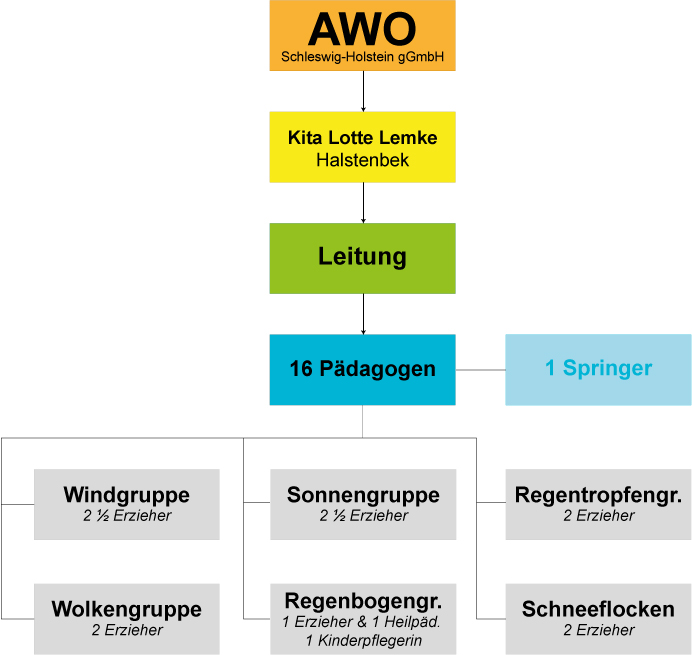
\includegraphics[width=\textwidth]{grafik/organigramm.jpg}
    \captionof{figure}[Organisationsstruktur der KiTa Lotte Lemke]{Organisationsstruktur der KiTa Lotte Lemke}
    \label{fig:organigramm}
  \end{center}
  
  
  \section{Die Besch�ftigten der Kindertagesst�tte Lotte Lemke}
    \begin{flushleft}
      Die Kita besch�ftigt 17 P�dagogen, eine Kitaleitung, eine Heilp�dagogin, drei Erzieher, acht Erzieherinnen, eine Kinderpflegerin und eine Sozialp�dagogische Assistentin, der �berwiegende Teil hat einen unbefristet Arbeitsvertrag. Zehn P�dagogen haben eine unbefristeten Vollzeitvertrag (39 Stunden). Des Weiteren haben drei P�dagogen einen unbefristeten Vertrag mit 30 Stunden und eine hat einen unbefristeten Vertrag mit 25 Stunden. Au�erdem gibt es noch zwei P�dagogen mit befristeten Arbeitsvertr�gen. Eine der beiden arbeitet 37 Wochenstunden und die andere jeweils neun Stunden die Woche.
      \\
      Neben den P�dagogen sind noch ein Koch und Hauswirtschafter, eine Haushaltshilfe, ein G�rtner, ein Hausmeister und zwei Reinigungskr�fte. Des Weiteren wird das Team von Praktikanten unterst�tzt.
    \end{flushleft}

  \section{Altersstruktur und Geschlechterverh�ltnis der P�dagogen}
    \begin{flushleft}
      Das Geschlechterverh�ltnis ist wie in vielen Kindertagesst�tten nicht sehr ausgeglichen, obwohl die Kindertagesst�tte Lotte Lemke auch mehr Frauen als M�nner besch�ftigt, hat sie mit drei m�nnliche P�dagogen und drei weiter M�nner die in der Kindertagesst�tte t�tig sind, mehr m�nnliches Personal als viele andere KiTas. 
      \\
      Das Team der KiTa Lotte Lemke ist vom Alter her recht gemischt, obwohl der Gro�teil in seinen Drei�igern ist, ist die Alterspannweite recht gro�; von Mitte zwanzig bis Anfang sechzig (vgl. Abbildung \ref{fig:altersverteilung})
    \end{flushleft}
    
    \begin{center}
      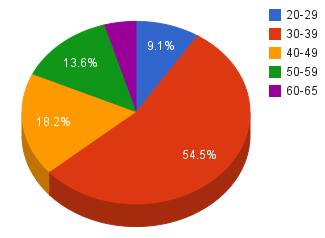
\includegraphics[width=0.55\textwidth]{grafik/altersverteilung.png}
      \captionof{figure}[Altersstruktur in der Kindertagesst�tte Lotte Lemke]{Altersstruktur in der Kindertagesst�tte Lotte Lemke}
      \label{fig:altersverteilung}
    \end{center}
    
    
  \section{Teamf�hrung}
    \begin{flushleft}
      Seit der �ffnung der Kindertagesst�tte Lotte Lemke hat Frau Baumann die Dienst- und Fachaufsicht und f�r die Abwesenheitsvertretung ist Frau Sanow zust�ndig. Zur Dienstaufsicht geh�ren unteranderem die Organisation und Planung der Arbeitsstunden. Sie erstellt mindestens sechs Wochen im Voraus den neuen Dienstplan. Hier bei werden Arbeitszeiten, Gruppenkonstellationen, Vorlieben f�r bestimmte Dienste wie Fr�h-und Sp�tdienste, Urlaube, Minusstunden und Mehrarbeit und wenn vorauszusehen auch Krankheit ber�cksichtigt. Der Plan h�ngt dann nach der Fertigstellung im B�ro aus und kann nach Absprache ver�ndert werden. Bei kurzfristigen �nderungen ist es wichtig dass der Kollege oder die Kollegin sich darum k�mmert das eine Vertretung f�r sie oder ihn verf�gbar. Der Dienstplan ist zwar verbindlich, da es aber bei einem Haus mit 16 P�dagogen immer wieder zu Ver�nderungen kommen kann, ist es unerl�sslich jeden Morgen auf den Dienstplan zu schauen. 
    \end{flushleft}
    
    \begin{flushleft}
      In der alle zwei Wochen stattfindenden Dienstbesprechung werden W�nsche, Anregungen, Organisatorisches, Ver�nderungen und Fachliches besprochen. Die Dienstbesprechungen beginnen nach Dienstschluss. Hier sollten nach M�glichkeit alle P�dagogen anwesend sein, wenn dies nicht der Fall ist, haben der oder die P�dagogin immer  die M�glichkeit es im Protokoll nachzulesen. Jede Dienstbesprechung wird von einem P�dagogenteam protokolliert und organisiert. Einmal im Jahr finden Personalgespr�che statt. Inhalte dieser Gespr�che sind p�dagogisches Verhalten, das Verhalten im Team und p�dagogische Fragen und Anliegen. Nat�rlich k�nne die Mitarbeiter jederzeit bei Anliegen und Vorkommnissen das Gespr�ch mit der p�dagogischen Leitung suchen. Dies ist auch ausdr�cklich gew�nscht.
    \end{flushleft}
    
    
  \section{Die Qualifikationen der Mitarbeiter}
    \begin{flushleft}
      Da die KiTa sich in verschiedene Fachbereiche aufteilt, hat jeder P�dagoge und jede P�dagogin ihren Fachbereich bzw. arbeitet mit ein oder zwei P�dagogen in diesem Fachbereich zusammen. Die P�dagogen und P�dagoginnen suchen sich den Fachbereich nach K�nnen und Interesse aus. Dem entsprechend kommt es auch vor das P�dagogen ihren Fachbereich entsprechende Fortbildungen besuchen und dann auch Elternabende dazu halten. Folgende Fachbereiche werden von den P�dagogen und P�dagoginnen abgedeckt: K�nstlerische Fr�hf�rderung, Werken und arbeiten mit Holz, Textiles Gestalten, Ern�hrung, Projektarbeit, Natur und Umwelt, Outdoor, Sprachf�rderung (\gls{Sismik}, \gls{Phonologie}), Wahrnehmung, Musikalische Fr�hf�rderung, \gls{Lernwerkstatt}, Graphomotorik, Bewegung (Sport, Tanzen), Kinderrat, Vollversammlung und Gruppenkonferenzen.
    \end{flushleft}    
    
  \section{Der Betreuungs- und der Stellenschl�ssel}
    \begin{flushleft}
      Das erforderliche Stundenkontingent der Kindertagesst�tte Lotte Lemke, umfasst die  Betreungsstunden,  die Vorbereitungszeiten und Elternarbeit, die Dienstbesprechungen, Urlaubstage, Fortbildungen sowie Krankheitstage (vgl. Anhang \ref{chap:anhang_2}). F�r die \enquote{Arbeit am Kind} steht der Kita f�r das ganze Jahr 20.352 Stunden zur Verf�gung. Die gesetzlichen Bestimmungen des Betreuungschl�ssel der Kindertagesst�tte Lotte Lemke liegen bei den Familiengruppen, bei einer Betreuung von 15 Kindern, bei 88 Stunden \enquote{Arbeit am Kind}, bei den Elementargruppen sind es 40 Betreuungsstunden, bei 20 Kindern. Des Weiteren haben die Outdoorgruppe und die Integrationsgruppe 40 Wochenstunden \enquote{Arbeit am Kind} bei 15 Kindern. Den Fr�hdiensten stehen dann noch 5 Stunden, der Mittagsdienst hat insgesamt 20 Stunden und der Sp�tdienst verf�gt �ber 2,5 Stunden die Woche (vgl. Anhang \ref{chap:anhang_3}). Die Abweichung der gesetzlichen Bestimmung von der tats�chlichen Aufteilung der Gruppen ist kaum zu vermeiden, da das Personal versucht den Kindern und Eltern, ihren Bed�rfnissen entsprechend, die bestm�gliche Betreuung zu bieten.
    \end{flushleft}
    
    
  \section{Arbeitszeiten}
    \begin{flushleft}
      Die Arbeitszeiten bei einer Vollzeitkraft (39 Stunden die Woche) k�nnen variieren, dies kann man an Hand der Abbildung sehen. Hier kann man einmal den Arbeitstag in den Kernzeiten 8-16 Uhr oder 9-17 Uhr sehen und dann noch mit Fr�h- und Sp�tdienst (vgl. Anhang \ref{chap:anhang_4}). Die Arbeitszeiten bei eine Teilzeitstelle mit 30,25 Stunden die Woche sind zum gr��ten Teil von 8:00-14:00 Uhr, die kann nat�rlich variieren ist aber meist nicht der Fall (vgl. Anhang \ref{chap:anhang_4}). Sowohl f�r die Teilzeit- wie auch f�r die Vollzeitkraft kommen noch die zweimal im Monat stattfindenden Dienstbesprechungen dazu.
    \end{flushleft}           
\newpage

% Kapitel 3: R�ume				
\chapter{R�ume}
  \section{Gruppenr�ume}
    \begin{flushleft}
      Das 1993 errichtete ebenerdig Geb�ude erstreckt sich �ber 350qm, mit einem Gel�nde von 3500qm und liegt in einer verkehrsberuhigten Zone. Die Gruppenr�ume haben alle die gleiche Grundausstattung, eine Hochebene, eine K�chenzeile mit Herd und Ofen, mindestens ein Sideboard, PVC Boden und vor jedem Gruppenraum befindet sich eine Garderobe. Den gro�en Unterschied machen die Themen der R�ume aus.
    \end{flushleft}
    
    \begin{flushleft}
      \textbf{Windgruppe}
      \\
      So ist die Windgruppe ein Projektraum und ist z.Z. im Zeichen der Indianer eingerichtet. Derzeitig geh�rt zur Einrichtung ein Tipi, Holzst�mme, Trommeln, eine Indianerverkleidungs- und Schminkecke und auf den drei Tischen sind immer wechselde Spiele, B�cher, Puzzle und Bastelangebote. Dass die Windgruppe eine Familiengruppe ist hat sie nicht nur zwei Waschr�ume, mit jeweils zwei Toiletten, sondern auch noch einen Wickelraum. Hier befinden sich ein Wickeltisch mit Waschbecken und die Windeln und Wechselw�sche sind hier auch zu finden. Au�erdem ist hier noch eine Kindertoilette, ein Kinderwaschbecken und ein Erwachsenenwaschbecken. Fast alle Gruppenr�ume haben einen Nebenraum, die Windgruppe hat in ihrem Nebenraum (Traumraum), der mit Decken, Kissen, Matratzen, Nachttischlampen, Vorh�ngen und einem kleinen Beistelltisch auf dem eine CD-Player steht gem�tlich gemacht wurde. Die Kinder k�nnen im Traumraum, schlafen, lesen bzw. sich B�cher angucken, und Musik und H�rspiele h�ren.
      
    \end{flushleft}

    \begin{flushleft}
      \textbf{Wolkengruppe}
      \\
      Die Wolkengruppe ist der Mal- und Gestaltungsraum. Die Kinder haben die M�glichkeit an den drei Sechsertischen, auf dem Boden oder an den Staffelein, mit Stiften, Tusche oder Fingermalfarbe ihrer Kreativit�t freien Lauf lassen. Auf einem kleinen Podest k�nnen sie dann auch Kneten und w�hrend der AG-Zeit k�nnen sie in der Holzwerkstatt, die sich in einem der zwei Nebenr�ume der Wolke befindet, an der Werkbank h�mmern und s�gen. Der zweite Nebenraum der Wolkengruppe ist das Kinderb�ro (vgl. Abschnitt \ref{sec:4_2}). Die Wolkengruppe hat einen gro�en Waschraum, mit zwei Toiletten und drei Waschbecken.
    \end{flushleft}

    \begin{flushleft}
      \textbf{Regentropfengruppe}
      \\
      Die Regentropfengruppe ist sowohl der Raum in der sich die \gls{Lernwerkstatt} (vgl. Anhang \ref{chap:anhang_6}) befindet, als auch andere Baumaterialen. Unteranderem k�nnen die Kinder eine Murmelbahn bauen, mit Autos spielen, aus Duplo und  Holzspielbausteinen k�nnen sie z.B. H�user oder St�dte bauen. Damit die Kinder nicht auf dem kalten PVC Boden sitzen m�ssen, gibt es drei Teppiche in der Gruppe. Einer der Teppiche ist ein Bauteppich. Sowie die Wolkengruppe hat auch die Regentropengruppe zwei Nebenr�ume. Einer der Nebenr�ume dient als Aufbewahrungsraum, unteranderm f�r die Lernwekstattmaterialien. Der zweite Nebenraum ist wie bei der Wolkengruppe, das Kinderb�ro (vgl. Abschnitt \ref{sec:4_2}). Die Regentropfen hat einen gro�en Waschraum, mit zwei Toiletten und drei Waschbecken.
    \end{flushleft}

    \begin{flushleft}
      \textbf{Sonnengruppe}
      \\
      Der Sonnengruppenraum ist sowohl ein Projektraum, als auch der Raum in der sich die Natur und Umwelt Materialien befinden. Das derzeitige Thema des Projektes ist Mittelalter, im Zuge dazu haben die Kinder w�hrend der AG-Zeit, die Hochebene in ein Schloss verwandelt. Das Projekt Mittelalter, steht noch recht am Anfang und ist deswegen noch ausbauf�hig. Zu dem Bereich Natur und Umwelt geh�ren B�cher, Spiele, Aquarien und Terrarien. In den Aquarien befinden sich nat�rlich verschieden Fische und in den Terrarien sind verschiedene Insekten sowie Spinnen, Schlangen und Eidechsen. Da die Sonnegruppe ebenfalls eine Familiengruppe ist, ist hier neben dem Waschraum mit zwei Toiletten und Waschbecken noch ein Wickelraum, der �hnlich ausgestattet ist wie der Wickelraum der Windgruppe. Au�erdem hat die Sonnengruppe zwei Nebenr�ume, einmal den Schlafraum und den Shiatsu-Raum (vgl. Abschnitt \ref{sec:4_2}). 
      Der Schlafraum der Gruppe ist mit drei Reisebetten ausgestattet.
    \end{flushleft}

    \begin{flushleft}
      \textbf{Regenbogengruppe}
      \\
      Der Gruppenraum der Regentropfengruppe, ist seit ca. einer Woche ein Rollenspielraum und befindet sich daher noch im Umstrukturierungsprozess. In den Nebenraum der Gruppe, ist nach einem gemeinsamen Beschluss der Kinder und P�dagogen der AWO KiTa,  die Puppenecke gezogen. Auf der Hochebene, der Gruppe, bewahrt die Gruppe Polster-Prismen auf. Spielen tun die Kinder damit nur unter der Hochebene. Die zwei Waschr�ume der Gruppe gehen nicht wie beiden anderen Gruppen von den Gruppenr�umen, sondern von der Garderobe ab.
    \end{flushleft}
    
  \newpage
  
  
  
  
  \section{Weitere R�ume der Kindertagesst�tte Lotte Lemke}\label{sec:4_2}
    \begin{flushleft}
      \textbf{Der Flur}
      \\
      Im Flur befindet sich eine Vielzahl von Dingen, zum einen befindet sich hier die K�nstlerecke. Diese grenzt sich durch zwei wei�e Regale und vier Sideboards, in denen Kisten mit allerlei Bastelsch�tzen stehen, vom Rest des Flures ab. In der Mitte dieses Bereiches stehen zwei Kindertische mit jeweils sechs St�hlen. Des Weiteren befindet sich rechts an der Wand ein rotes Metallregal mit Fingerfarbe und daneben steht ein ein h�lzernes Sideboard mit Papier zum Malenund links neben dem Metallregal steht ein wei�er Tisch. In der K�nstlerecke k�nnen Kinder in der AG oder Freispielzeit, mit der P�dagogin die f�r den Fachbereich zust�ndig ist, aktiv werden. Des Weiteren befinden sich eine Themenecke, die derzeitig umgestaltet wird, ein B�llebad, eine Leseecke und Geburtstagstisch ein Elterncaf� im Flur. Das Elterncaf� befindet sich gegen�ber vom B�llebad (vgl. Anhang \ref{chap:anhang_6}), den Eltern steht eine Sitzgruppe mit einem Tisch zur Verf�gung. T�glich werden hier Kaffee, Tee und Wasser f�r die Eltern bereitgestellt. Das Elterncaf� wird h�ufig w�hrend der Eingew�hnungsphase genutzt.
    \end{flushleft}
    
    
    \begin{flushleft}
      \textbf{B�ro}
      \\
      Das Erwachsenenb�ro ist mit zwei Schreibtischen und Schreibtischst�hlen, mit einem Computer und einem Laptop, mehreren Aktenregalen, zwei Drucker und Kopierer und Sideboards in denen unteranderem Digitalkameras und Fieberthermometer aufbewahrt. Au�erdem dem stehen dort noch zwei Regale mit Spielsachen f�r die Kinder. Das B�ro steht den Kinder jederzeit zum Spielen zur Verf�gung.
    \end{flushleft}
    
    \begin{flushleft}
      \textbf{Kinderb�ro}
      \\
      Das Kinderb�ro liegt zischen dem Gruppenr�umen der Regentropfen und der Wolke. Die Kinder k�nnen sich hier ein- bis zweimal t�glich, an der Bildertafel (vgl. Abschnitt \ref{sec:7_4}) eine AG aussuchen. Gegen�ber von der Bildertafel liegt eine blau Matratze auf die sich die Kinder w�hren der AG-Besprechung setzen k�nnen. Au�erdem k�nnen sie im Kinderb�ro ihre Schreibeordner (vgl. Abschnitt \ref{sec:7_7}) einsehen. Die Ordner stehen in wei�en Regalen, in f�r Kinder gut erreichbarer H�he.
    \end{flushleft}
    
    \begin{flushleft}
      \textbf{Shiatsu-Raum}
      \\
      Einer der Nebenr�ume der Sonnengruppe wird als Shiatsu-Raum genutzt. In dem Raum liegt eine Matratze die den Gro�teil des Raumes einnimmt. Des Weiteren steht in dem Raum ein Rollwagen, der an einen Teewagen erinnert, auf ihm befinden sich Klangschalen, CD-Player, CD's mit Entspannungsmusik und verschiedene Massageutensilien. W�hrend der AG-Zeit und am Nachmittag wird hier \gls{Shiatsu} angeboten. Am Nachmittag geschieht dies durch eine Shiatsu-Therapeutin. Die Eltern m�ssen f�r diese Einzelbehandlung \EUR{45} pro Mal bezahlen.
    \end{flushleft}
    
    \begin{flushleft}
      \textbf{Matschraum}
      \\
      Der Matschraum ist ein wei� gekachelter Raum, mit einer gro�en Fl�che auf der vier Plantschbecken Platz finden. Die Kinder k�nnen nackt oder in Badehose, in Begleitung eines P�dagogen in den Raum. Je nach Angebot k�nnen die Kinder sich, die W�nde und den im Raum vorhanden Spiegel z.B. mit Fingerfarbe, Duschbad oder Duschpeeling einseifen. Anschlie�end gehen sie dann in die Wasser bef�llten Plantschbecken. Hier haben sie dann die M�glichkeit mit diversen Badespielsachen zu spielen. Des Weiteren sind eine Toilette, eine Dusche und ein Waschbecken in diesem Raum.
    \end{flushleft}
    
    \begin{flushleft}
      \textbf{Kindercaf�}
      \\
      Im Kindercaf� k�nnen die Kinder- wie in Abschnitt \ref{sec:7_8} weiter erl�utert wird- ihre Mahlzeiten einnehmen. Den Kindern stehen hierf�r mehrere Tische und St�hle zur Verf�gung. An den W�nden h�ngen selbstgemalte und -gestaltete Bilder. In der Mitte des Raumes steht ein wei�bemalter Baum, der von Tischen umringt ist, an dem selbstgebasteltes und eine Lichterkette h�ngt. All dies verleiht dem Raum Gem�tlichkeit.
    \end{flushleft}
    
    \begin{flushleft}
      \textbf{Turnhalle}
      \\
      In der Halle k�nne die Kinder mehrmals am Tag ihrem Bewegungsdrang ausleben. Die Halle ist ausgestattet mit mehreren dicken und d�nnen blauen Matten, einer Kletterwand, einer Sprossenwand, zwei B�nken, einem Kastenwagen und einem kleinen Kasten. Au�erdem finden sich im Nebenraum der Turnhalle B�lle, Seile, Rollbretter, Schwungt�cher usw.. Diese Dinge k�nnen auf Wunsch rausgeholt werden.
    \end{flushleft}
 

  \section{Das Au�engel�nde der KiTa Lotte Lemke}
    \begin{flushleft}
      Das Au�engel�nde der KiTa Lotte Lemke erstreckt sich �ber ca. 3000qm. Auf beiden Seiten des Geb�udes wird den Kindern die M�glichkeit geboten zu spielen. Rechts vom Geb�ude wurden im letzten Jahr, in Zusammenarbeit einiger Eltern, eine neue Spiellandschaft errichtet. Die Umgestaltung des Gel�ndes, war ein partizipativer Prozess an dem die Kinder, P�dagogen, Landschaftsarchitekten und externe Moderatoren beteiligt waren. Zu der Spiellandschaft geh�rt eine Spielplatzpumpe mit Matschanlage, drei Turnstangen, eine Sandkiste in der die  Kletterlandschaft die wie ein Piratenschiff aussieht steht und ein H�gel. Die Fahrzeuge, die mitgebracht oder aus dem Schuppen geholt werden, k�nnen auf dem gepflasterten Weg gefahren werden. Auf der linken Seite des Geb�udes ist der gr��te Teil der Fl�che Rasen. Es bietet sich sehr an hier Fu�ball zu spielen. Au�erdem stehen eine Mehrkindschaukel und mehrere Obstb�ume auf dem Gel�nde.
    \end{flushleft}
           
\newpage

% Kapitel 4: Kinder der Regenbogengruppe				
\chapter{Die Regenbogengruppe}
  \section{Anzahl, Geschlecht und Aufenthaltzeit}
    \begin{flushleft}
      In der Regenbogengruppe, die eine Integrationsgruppe ist werden zur Zeit 16 Kinder von einer Erzieherin, einer Heilp�dagogin und einer Kinderpflegerin betreut. Von den 16 Kindern drei Kinder �ber drei mit besonderen F�rderbedarf mit juristischer Anerkennung und ein Kind unter drei Jahren mit besonderem F�rderbedarf aber gegenw�rtig noch ohne juristische Anerkennung. Von den derzeitig 16 Kindern sind acht M�dchen und acht Jungen. Die Betreungszeiten der Kindern sind sehr unterschiedlich.  F�nf Kinder haben einen Platz von 8---12 Uhr, sieben Kinder haben einen Platz von 8---14 Uhr und vier Kinder werden nach Bedarf der Eltern an einigen Tagen von 8---12 betreut und an anderen von 8---14 Uhr. Allen Eltern steht frei, nach Bedarf Betreuungstunden f�r ihre Kinder dazu zu buchen. Der Gro�teil der Regenbogen-Kinder ist mit zwei oder drei Jahren in die Kindertagesst�tte Lotte Lemke gekommen. Sieben der Kinder der Regenbogengruppe waren zuvor bereits ein Jahr in der  Nachmitttagsgruppe (12---17 Uhr oder von 14---17 Uhr) und sind im August 2011 in die Regenbogengruppe gewechselt. Ein Kind ist seit seinem ersten Lebensjahr in der Gruppe. Au�erdem sind drei der Kinder erst mit vier Jahren in die Kindertagesst�tte Lotte Lemke gekommen.
    \end{flushleft}
    
    
  \section{Altersstruktur}
    \begin{flushleft}
      Das j�ngste Kind ist ein M�dchen, sie ist dieses Jahr zwei geworden. Da sie einen besonderen F�rderbedarf hat, ist sie nicht wie �blich bei Kindern unter drei in die Familiengruppe, sondern um dem besonderen Bedarf gerecht zu werden, in die Integrationsgruppe gekommen. Hier kann durch die Anzahl der Betreungskr�fte und der Heilp�dagogin ihr eher gerecht werden. Im Alter von drei Jahren sind zwei Jungen und ein M�dchen. Des weiteren gibt es drei vierj�hrige Jungen und drei vierj�hrige M�dchen. Vier Kinder der Regenbogengruppe sind f�nf Jahre alt, davon sind drei M�dchen und zwei Junge. Au�erdem gibt es noch zwei sechsj�hrige in der Gruppe, jeweils ein Jungen und ein M�dchen.
    \end{flushleft}           
\newpage

% Kapitel 5: Familie				
\chapter{Die Familien der Regenbogenkinder}
  \section{Die Familienkonstellation}
    \begin{flushleft}
      Fast alle Kinder der Regenbogengruppe leben in der traditionellen \enquote{Mutter- Vater-Kind-Familie}. Die Eltern eines M�dchens leben getrennt und sie lebt mit ihrer Mutter und Gro�mutter zusammen. Die Mehrheit der Kinder in dieser Gruppe,haben ein oder mehr Geschwister. Nur vier der Regenbogen-Kinder haben keine Geschwister. Von den Kindern mit �lteren Geschwistern besuchen zwei die Kita Lotte Lemke.  Einer geht ebenfalls in Regenbogengruppen und eine ist in einer der Familiengruppen. Alle anderen Kinder haben �ltere Geschwister die schon zur Schule gehen. Bei den Kindern mit j�ngeren Geschwistern ist es �hnlich. Hier besuchen ebenfalls zwei Geschwisterkinder die Kita. Eine davon ist in der Regenbogengruppe und der andere besucht eine der Elementargruppen. Alle anderen haben Geschwister, die noch nicht den Kindergarten besuchen. Familien mit mehr als zwei Kindern finden sich in drei F�llen. In zweien der F�lle sind die Geschwister �lter und in einem sind sie j�nger.
    \end{flushleft}

  \section{Berufst�tigkeit der Eltern}
    \begin{flushleft}
      Ein Gro�teil der Eltern ist berufst�tig bzw. ein Elternteil ist berufst�tig. In den meisten Familien kann man eine Tendenz zur klassischen Rollenverteilung erkennen. Acht M�tter haben sich aufgrund von kleineren Geschwistern bewusst entschieden noch nicht zu arbeiten, im Gegenzug dazu sind 14 V�ter berufst�tig und vollzeitbesch�ftigt. Von den berufst�tigen M�ttern, sind zwei vollzeitbesch�ftigt und drei teilzeitbesch�ftigt. Eine der berufst�tigen M�tter ist aufgrund ihrer Krebserkrankung bis auf Weiteres krankgeschrieben. Leider sind z.Z. bei zwei Kindern jeweils ein Elternteil ungewollt ohne Arbeit. 
    \end{flushleft}
    
    
  \section{Wohnsituation und Wohnort der Kinder}
    \begin{flushleft}
      Die meisten Kinder, der Regengruppe haben eine stabile Sozialelage. 
      Sie wohnen mit ihren Familien in Einfamilienh�usern mit Garten oder in Mehrfamilienh�usern und haben ihr eigenes Zimmer, ausgestattet mit den verschiedensten Spielsachen z.B. eine elektrische Eisenbahn, einen Kaufmannsladen, Murmelbahn oder auch ein Mischpult. Fast alle Kinder der Regenbogengruppe wohnen in der Gemeinde Halstenbek, zum Teil werden die Kinder zu Fu� oder mit dem Fahrrad in die Kita gebracht, aber der Gro�teil wird mit dem Auto gebracht.
    \end{flushleft}


  \section{Migration und besondere Bed�rfnisse}
    \subsection{Die F�rderung besonderer Bed�rfnisse}
      \begin{flushleft}
        Aufgrund des Integrationsstatus der Regenbogengruppe - wie bereits in 4.1 erw�hnt - sind hier drei mit Kinder �ber drei mit besonderen F�rderbedarf mit juristischer Anerkennung und ein Kind unter drei Jahren mit besonderen F�rderbedarf aber gegenw�rtig noch ohne juristischer Anerkennung. Au�erdem bekommen noch weitere Kinder eine besondere F�rderung. Derzeitig wird getestet, ob zwei Jungen eine Hochbegabung haben, diese Kinder haben besondere Bed�rfnisse, auf die eingegangen werden muss. Insbesondere erfolgt die Begleitung der Kinder mit besonderen Bed�rfnissen durch die Heilp�dagogin, die ein gro�es Augenmerk auf die Selbstverst�ndlichkeit im  Umgang mit Behinderungen jeglicher Art legt. \enquote{Jedes Kind ist besonders in seiner Art.} (Zitat: Britta Henningsen)
      \end{flushleft}

      \begin{flushleft}
         Da es eine Vielfalt von besonderen Bed�rfnissen gibt, arbeiten die P�dagogen mit einer Vielzahl an Therapeuten zusammen. Darunter fallen Ergotherapeuten, L�gop�den, Kinderpsychologen und Physiotherapeuten. Au�erdem wird mit verschiedenen Instituten, wie dem Werner Otto Institut und dem Fleming Institut, zusammengearbeitet \citep[vgl.][]{Integration2007}. Es besteht die M�glichkeit, dass externe Spezialisten in die Kindertagesst�tte kommen.
      \end{flushleft}

     
    \subsection{Migration und Sprachf�rderung}
      \begin{flushleft}
        Drei Kinder der Regenbogenkinder haben einen Migrationshintergrund (indisch, irisch und japanisch). Sie erhalten einmal pro Woche besondere Sprachf�rderung durch \gls{Sismik} (Sprachverhalten und Interesse an Sprache bei Migrantenkindern in Kindertageseinrichtungen). Diese F�rderung findet durch zwei p�dagogische Mitarbeiter, die beide eine Weiterbildung im Bereich Sprachf�rderung haben, statt. Dies findet zweimal die Woche w�hrend der AG-Zeit statt. Eine P�dagogin begleitet die 3 � j�hrigen bis 5 j�hrigen und eine andere die Kinder die dieses Jahr zur Schule kommen.
      \end{flushleft}           
\newpage

% Kapitel 6: P�dagogische Arbeit				
\chapter{P�dagogische Arbeit}
  \section{Der p�dagogische Auftrag der KiTa Lotte Lemke}\label{sec:7_1}
    \begin{flushleft}
        Der p�dagogische Auftrag der KiTa Lotte Lemke bezieht sich unteranderem auf den Bildungsauftrag vn INFANS-Konzept f�r Fr�hp�dagogik vom Institut f�r angewandte Sozialforschung / Fr�he Kindheit e.V.. Hier geht es vorallem darum, dass lernen ein  Lebenslanger Prozess ist, der von jedem Menschen mitbestimmt wird. Doch f�r eine gelungene Entwicklung sind Menschen abh�ngig,  von der Interaktion mit anderen. F�r das Kind hei�t das, es braucht eine Bindungsperson, um die Welt erkunden zu k�nnen \citep[vgl.][]{paBild2009}. Darauf aufbauend ist dem Personal der KiTa Lotte Lemke sehr wichtig, dass sich jedes Kind wohl und geborgen in der KiTa f�hlt und Vertrauen zu den P�dagogen aufbaut \citep[vgl.][]{paBild2009}. Jedem Kind wird Wertsch�tzung und Anerkennung entgegengebracht.
        \\
        Au�erdem ist dem KiTa-Team wichtig die Kinder mit wichtigen Attributen wie Selbstvertrauen, Selbstbewusstsein, Selbstst�ndigkeit, Konfliktf�higkeit, Entscheidungsf�higkeit, Toleranz und Akzeptanz, auszustatten \citep[vgl.][S.~12ff]{padZiel2000}. Des Weiteren sind die F�rderung der Kreativit�t und Phantasie f�r die individuelle Entwicklung und die F�rderung zur Entwicklung des Sozialverhaltens  wichtige Bestandteile des p�dagogischen Auftrags \citep[vgl.][S.~12ff]{padZiel2000}. \enquote{Hilf mir es selbst zu tun.} (Zitat: Maria Montessori zitiert nach \citep[vgl.][]{paBild2009}) 
    \end{flushleft}
  
  
  \section{Das Konzept und die Besonderheiten der KiTa}
    \begin{flushleft}
      Die KiTa Lotte Lemke die Schwerpunkten in ihrer Arbeit sind sehr verschieden unteranderem arbeitet die Kindertagesst�tte nach dem Situationsansatz. Die P�dagogen sind zu dem Entschluss gekommen, dass das gruppen�bergreifende Arbeiten die Merkmale des Situationsansatzes am Besten aufgreift. Durch Angebote, Projekte und AG's eignen sich die Kinder wichtige Attribute (vgl. Abschnitt \ref{sec:7_1}) an \citep[vgl.][S.~15f]{Sitans2000}.
    \end{flushleft}


    \begin{flushleft}
      Zudem ist das Thema Partizipation ein wichtiger Baustein im KiTa-Alltag. \enquote{Unter Partizipation verstehen wir die Mitbestimmung und Beteiligung der Kinder im Alltag.} (Zitat nach \citep[vgl.][]{Patiz2011}) Die Mitbestimmung ihres KiTa-Alltags erleben die Kinder t�glich. Ich m�chte dies an der t�glichen Bildertafel-Situation erl�utern. Die Kinder k�nnen  t�glich zwischen verschiedenen Angeboten, Projekten und AG's w�hlen. Dabei treffen sie nicht nur eigene Entscheidungen, sondern sie m�ssen sie sich auch untereinander abstimmen, da alle Angebote, Projekte und AG's nur eine bestimmte Kapazit�t haben. Hilfestellung von den P�dagogen sind hier dann auch angebracht \citep[vgl.][]{Patiz2011}. \enquote{Wir (P�dagogen) bestimmen, was Ihr (Kinder) bestimmen d�rft!} (Zitat nach \citep[vgl.][]{Patiz2011}) Wichtig ist zu erw�hnen das Partizipation nur im Zusammenspiel mit der Verfassung funktioniert (vgl. Anhang \ref{chap:anhang_5}). Die Verfassung, die 2007 in Kraft trat, beinhaltet die Partizipationsrechte der Kinder \citep[vgl.][]{Verfas2008}. 
    \end{flushleft}
    
    
  \section{Tagesablauf}
    \begin{flushleft}
      So k�nnte ein Tag in der Kindertagesst�tte Lotte Lemke aussehen.
    \end{flushleft}
    \begin{center}
      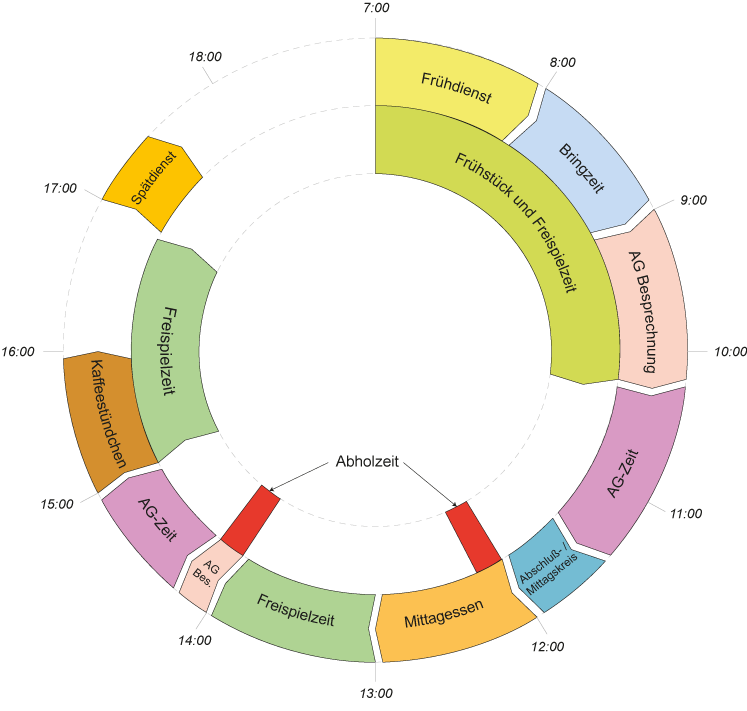
\includegraphics[width=0.82\textwidth]{grafik/tagesablauf.png}
      \captionof{figure}[Tagesablauf der Kindertagesst�tte Lotte Lemke]{Ein Beispiel Tagesablauf der Kindertagesst�tte Lotte Lemke}
      \label{fig:tagesablauf}
    \end{center}
    
  
  \section{Elternarbeit}\label{sec:7_4}
    \begin{flushleft}
      Die Elternzusammenarbeit ist ein wichtiger Punkt in der KiTa Lotte Lemke. Sie beinhaltet Erstgespr�che, Elterngespr�che und Elternabende \citep[S.~29]{Eltzuar2000}.
    \end{flushleft}
    
    \begin{flushleft}
      \textbf{Elterngespr�che}
      \\ 
      Der Informationsaustausch �ber den Entwicklungsstand des Kindes erfolgt unteranderem durch Elterngespr�che. Diese k�nnen jederzeit, nach Terminabsprache, gef�hrt werden \citep[vgl.][S.~28f]{Eltzuar2000}. Die P�dagogen bereiten sich hierf�r mit der Entwicklungsmappe des jeweiligen Kindes vor. In der Mappe befinden sich Kinderbeobachtungsb�gen (KBB) (vgl. Anhang \ref{chap:anhang_7}), Soziogramme (vgl. Anhang \ref{chap:anhang_8}), Kinderfrageb�gen (vgl. Anhang \ref{chap:anhang_9}), Entwicklungsb�gen. Au�erdem stehen die P�dagogen im st�ndigen dialogischen Austausch mit ihren Kollegen. Vor und nach Elterngespr�chen wird sich mit der Kitaleitung ausgetauscht, diese steht den jeweiligen P�dagogen jederzeit mit Rat und Tat zur Seite. Elterngespr�che sind nicht nur ein Informationsaustausch, sie dienen auch zur Beratung und wenn n�tig auch zur Vermittlung an weitere Institutionen \citep[vgl.][S.~28f]{Eltzuar2000}.
    \end{flushleft}
    
    \begin{flushleft}
      \textbf{Elternabende}
      \\
      In der KiTa Lotte Lemke werden Gesamtelternabende und Themenelternabende nach Bedarf und Interesse angeboten. Wohingegen gruppeninterne Elternabende zweimal im Jahr stattfinden. W�hrend dieser Elternabende werden (KiTa) politische, p�dagogische und inhaltliche Themen besprochen \citep[vgl.][S.~28f]{Eltzuar2000}.
    \end{flushleft}
 

  
  \section{Die Inhalte und der Umfang der Vor- und Nachbereitung}
    \begin{flushleft}
      Den P�dagogen stehen je nach Stundenanzahl drei bis f�nf Stunden Vor- und Nachbereitung zur Verf�gung. Diese nutzen sie um KBBs, Soziogramme und Entwicklungsb�gen (vgl. Anhang \ref{chap:anhang_8}) zu erstellen. Zudem schreiben sie \enquote{Lernngeschichten} f�r die Kinder, diese kommen dann in die Schreibeordner der Kinder.
    \end{flushleft}

    \begin{flushleft}
      \textbf{Schreibeordner}
      \\ 
      Jedes Kind hat im Kinderb�ro einen Aktenorder stehen, in welchem �ber das Jahr nach Wunsch des Kindes verschiedene Dinge gesammelt werden. Die Ordner stehen in einer f�r Kinder gut erreichbaren H�he, so dass sie jederzeit angeguckt werden k�nnen. In dem Schreibeordner befinden sich unteranderem Lerngeschichten, die auf der Grundlage von Beobachtungen und Fotos, von einem Erzieher pers�nlich f�r das Kind geschrieben wurden.  Nach Wunsch k�nnen die Kinder auch Gemaltes oder Gebasteltes in ihren Schreibeordner heften.
    \end{flushleft}

    

    
  \section{Die Ausfl�ge und Reisen}
    \begin{flushleft}
      \textbf{Ausfl�ge}
      \\
      Ausfl�ge sind bestandteil des t�gliche KiTa-Alltags. Dies wird den Kindern durch die Outdoorgruppe erm�glicht. T�glich gehen zwei bis vier Kinder aus den f�nf Vormittags- und Ganztagsgruppen mit. Bei der Ausflugsplanung entscheiden die Kinder mit wem und an welchen Tagen sie mitgehen. Hierbei wird versucht, den W�nsche der Kinder gerecht zu werden \citep[vgl.][S.~19]{KonzReUb2000}. Die Ausfl�ge gehen von um 9:00 Uhr --- 12:00 Uhr und f�hren die Kinder in die nahe und ferne Umgebung von Halstenbek. F�hrt es die zwei Erzieher und die 15 Kinder bis nach Hamburg.
    \end{flushleft}

    \begin{flushleft}
      \textbf{Reisen}
      \\
      Reisen finden hingegen alle zwei Jahre statt. Die Planung der Reise ist ein langer Prozess, den Kinder, P�dagogen und Eltern gemeinsam tragen. Es wird �berlegt wohin man reisen kann, so dass es sich auch alle leisten k�nnen. Wie kommt man da am Besten hin? Welches Kind m�chte bei welchem Erzieher bzw. welcher Erzieherin �bernachten. Dieser Prozess wird durch den Kinderrat dokumentiert, protokolliert und beschlossen \citep[vgl.][S.~19]{KonzReUb2000}.
    \end{flushleft}
    
    
  \section{Qualit�tssicherung}\label{sec:7_7}
    \begin{flushleft}
      Eine  Qualit�tssicherung ergibt durch den regen Austausch der P�dagogen und P�dagoginnen untereinander und mit der p�dagogischen Leitungskraft. Wie bereits in 1.5 erw�hnt, arbeiten die  Mitarbeiter in Kooperation mit Mitarbeitern der anderen AWO Schleswig Holstein gGmbH Kindertagesst�tten, in Qualit�tszirkeln um kontinuierlich das Angebote f�r Kinder und Familien zu verbessern.
    \end{flushleft}
    
    
  \section{Ern�hrung und Hygiene}\label{sec:7_8}
    \subsection{Ern�hrung in der Kita}
      \begin{flushleft}
        Ein wichtiger Bestandteil einer gesunden Entwicklung, ist eine ausgewogene und abwechslungsreiche Ern�hrung. In der Kindertagesst�tte wird dies unteranderem durch den hauseigenen Koch gew�hrleistet.T�glich wird von ihm frisch, abwechslungsreich, ausgewogen und kindgerecht gekocht, dazu geh�rt auch mal etwas S��es. Au�erdem ist er darauf bedacht, die verschieden Essgewohnheiten und Di�ten zu ber�cksichtigen \citep[vgl.][S.~27]{KonzEr2000}. Der Aufgabenbereich des Kochs umfasst mehr als nur das Zubereitung der Speisen, er k�mmert sich auch um die organisatorische Planung, die Zusammenstellung der Speisen und den Einkauf \citep[vgl.][]{ErHy2006}.
      \end{flushleft}
      
    \subsection{Die verschiedenen Mahlzeiten}
      \begin{flushleft}
        \textbf{Das Fr�hst�ck}
        \\
        Die Kinder in der Kita Lotte Lemke haben die M�glichkeit ihr Fr�hst�ck zwischen 7:00 und 10:15 Uhr im Kindercafe einzunehmen. Meistens gehen sie mit ihrer Brottasche ins Kindercafe und  machen es sich mit einem oder mehreren Freunden gem�tlich.  Hier wird sich dann unterhalten, gegessen und auch mal nach Wunsch Essen getauscht \citep[vgl.][]{ErHy2006}. Kinder mit Allergien, Diabetiker oder mit anderen Einschr�nkungen wissen, dass sie davon ausgeschlossen sind, dies wurde mit den  Kindern  Zuhause und in der Zuhausegruppe thematisiert. Au�erdem wurden alle P�dagogInnen im Haus dar�ber informiert. Mitunter haben die Kinder aus der Zuhausegruppe  eine Auge darauf, wer was essen darf. Die Kinder d�rfen sich bei ihrem Fr�hst�ck soviel Zeitlassen wie sie wollen. Wenn sie fertig sind, k�mmert sich jedes Kind eigenst�ndig darum, dass sein Geschirr und Besteck auf den Teewagen kommen \citep[vgl.][]{ErHy2006}. Der eventuell produzierte M�ll, wird entweder zur�ck in die Brotdose bzw. Brottasche oder in die vor dem Kindercaf� stehenden M�lleimer getan. Da in der Kita- wie vieler Orts --- recycelt wird, stehen links von T�r des Kindercaf�s, w�hrend der Fr�hst�ckszeit vier M�lleimer (Plastikm�ll, Papierm�ll, Biom�ll, Restm�ll). Die Aufsicht im Kindercaf� ist durch die Gruppendienste geregelt, Montags sind z.B. die P�dagogen der Windgruppe f�r die Aufsicht des Kindercaf�s zust�ndig (Die t�glich rotierende Aufsichtspflicht der P�dagogen betrifft nicht nur das Kindercaf�, sondern auch die Turnhalle und das Au�engel�nde). Im Kindercaf� steht den Kindern t�glich zu jeder Zeit ein frischer Obst- bzw. Gem�seteller, unges��ter Tee, Milch, Mineralwasser zur freien Verf�gung \citep[vgl.][]{ErHy2006}.
      \end{flushleft}

      \begin{flushleft}
        \textbf{Das Mittagessen}
        \\
        Das Mittagessen wird t�glich frisch zubereitet und um 12:00 Uhr angeboten. Die meisten Gruppen, essen in ihrem Gruppenraum, die Regentropfengruppe und die Schneeflocken essen gemeinsam im Kindercaf�. Die Kinder k�nnen selber entscheiden ob sie mitessen wollen oder nicht, wenn sie wissen dass es ihnen nicht schmeckt m�ssen sie nicht probieren. Neue Speisen werden meistens probiert,wenn es aber nicht schmeckt k�nnen die Kinder ihren Teller abr�umen und ihre Brotdose holen. Die Kinder nehmen Einfluss auf die Mahlzeiten die ihnen serviert werden- nach jedem Essen wird eine Umfrage gemacht, wie das Essen jedem einzelnen geschmeckt hat. Hierbei k�nnen die Kinder zwischen gut, mittel und schlecht entscheiden. Dies wird dann auf einer Liste mit drei unterschiedlichen Smilies (vgl. Anhang \ref{chap:anhang_10}), f�r jeden Wochentag festgehalten. Nach dem Essen k�nnen die Kinder ihre Z�hne putzen.
      \end{flushleft}

      \begin{flushleft}
        \textbf{Das Kaffeest�ndchen}
        \\
        Das Kaffeest�ndchen f�ngt um 15 Uhr gleich nach der zweiten AG- Zeit an. Die Kinder und P�dagogInnen bekommen hier die M�glichkeit eine selbst mitgebrachte Kleinigkeit im Kindercaf� zu essen. Da das Kaffeest�ndchen �hnlich abl�uft wie das Fr�hst�ck, werde ich es nicht weiter erl�utern.
      \end{flushleft}
      
    \subsection{Hygiene in der Kita}
      \begin{flushleft}
        Die Kindertagesst�tte Lotte Lemke unterliegt --- wie alle Kindertagesst�tten- den Richtlinien der HACCP (Hazard Analysis and Critical Control Points; deutsch Gefahrenanalyse und kritische Lenkungspunkte) und des Infektionsschutzgesetzes �34 IJSG \citep[vgl.][]{ErHy2006}.
      \end{flushleft}
      
      

      \begin{flushleft}
        \textbf{Personelle Schulung} 
        \\
        Die Belehrungen des Infektionsschutzgesetzes und Hygienevorschriften erfolgt von dem Tr�ger (AWO) und wird j�hrlich aufgefrischt. Der Koch bekommt zus�tzlich viertelj�hrlich beim Wirtschaftertreffen, neue Anregungen wie die Hygieneverordnung in Kindertagesst�tten umgesetzt werden kann \citep[vgl.][]{ErHy2006}.
      \end{flushleft}


      \begin{flushleft}
        \textbf{Die Umsetzung in der K�che und im Wirtschaftsraum}
        \\
        Eine der wichtigsten Regeln f�r die K�che ist, \enquote{Eltern und Kinder d�rfen die K�che nicht betreten!} \citep[vgl.][]{ErHy2006}
        Um den Richtlinien der HACCP gerecht zu werden muss die Kerntemperatur der Speisen mindestens 65�C betragen. Au�erdem wird von jeder zubereiteten Speise eine Probe entnommen, diese wird dann mit Datum gekennzeichnet und f�r 14 Tage eingefroren. Dies passiert auch mit den Speisen, die Eltern f�r Feste zubereiten und mitbringen. Da die Gefahr beiLebensmittel bei denen die K�hlkette unterbrochen wurde und von rohen Eiern, Fisch oder Fleisch zu hoch ist --- sind sie verboten \citep[vgl.][]{ErHy2006}.
      \end{flushleft}


      \begin{flushleft}
        \textbf{Die Umsetzung in den Gruppen und beim Essen}
        \\
        Die Tische, Arbeitsfl�chen und Wickeltische werden jeden Morgen von einem P�dagogen desinfiziert. Au�erdem werden einmal die Woche die Handt�cher gewechselt und gereinigt, die Reinigung gilt auch f�r die Zahnputzbecher und -b�rsten. Die Zahnb�rsten werden nach Bedarf gewechselt \citep[vgl.][]{ErHy2006}.
      \end{flushleft}

                 
\newpage

% Kapitel 7: Umfeld der Praxiseinrichtung				
\chapter{Das Umfeld der Kindertagesst�tte Lotte Lemke}
  \section{Daten und Fakten der Gemeinde Halstenbek und des Kreis Pinneberg}
    \begin{flushleft}
      Die Kindertagesst�tte Lotte Lemke liegt in der Amtsfreien Gemeine Halstenbek. In der Gemeinde leben 16.744 Menschen und sie besteht aus den zwei Ortsteilen Halstenbek und Krupunder. Ihre Gesamtfl�che umfasst ca.1.260 ha und liegt im gr��ten Baumschulgebiet weltweit. Durch die g�nstige Lage der Gemeinde- sie grenzt unmittelbar an die Hansestadt Hamburg - ist sie sowohl ein beliebter Wohnort, als auch Gewerbestandort \citep[vgl.][]{Halstenbek2012}.
      Des Weiteren befinden sich sechs Kindertagesst�tten \citep[vgl.][]{HalstenbekKita} und vier Schulen in Halstenbek \citep[vgl.][]{HalstenbekSchule}. Eine der vier Schulen ist die 1994 er�ffnete Japanische Schule. Diese hat einen Zuzug  japanischst�mmigender Familien beg�nstigt \citep[vgl.][]{JapSchule}.
      \\
      Halstenbek liegt im Kreis Pinneberg dieser umfassen acht St�dte, drei amtsfreie Gemeinden und 38 amtsangeh�rige Gemeinden.
      Der Kreis ist einer der elf Kreise im Bundesland Schleswig-Holstein. Zudem ist der Kreis Pinneberg teil der Metropolregion Hamburg. Er grenzt im S�den an die Elbmetropole Hamburg und dem nieders�chsischen Landeskreis Stade. �stlich vom Kreis Pinneberg liegt der Kreis Segeberg und im Norden grenzt er an den Kreis Steinburg.
    \end{flushleft}


    \begin{flushleft}
      Obwohl das Kreisgebiet, bezogen auf die Fl�che 664 qkm der kleinste Kreis ist, ist er wiederum bezogen auf die Bev�lkerungsdichte 304.065 Einwohner der gr��te Kreis \citep[vgl.][]{KPinneberg2012}. Die Bev�lkerungsstruktur im Kreis Pinneberg weicht von der Schleswig-Holsteins in einigen Bereichen ab. So sind zwar die Zahlen der unter 18 J�hrigen und der �ber 65 J�hrigen  mit 17,6\% und 21,3\% fast identisch mit dem schleswig-holsteinischen Durchschnitt, doch bei der Arbeitslosenquote kann man schon Unterschiede erkennen: die Arbeitslosenquote vom Kreis Pinneberg liegt bei 5,6\% und in gesamte Schleswig-Holstein bei 6,9\%. So liegt das durchschnittliche Jahreseinkommen mit \EUR{20 200} nicht viel h�her als der Durchschnitt vom gesamten Schleswig-Holstein mit \EUR{18 446}, aber das erwirtschafte Bruttoinlandprodukt weicht wiederum stark ab, der Kreis Pinneberg erwirtschaftet 72 097 Millionen Euro, wohingegen das gesamte Schleswig-Holstein nur 58 092 Millionen Euro erwirtschaftet. Ein Grund daf�r k�nnten die Baumschulen sein und deren europaweiter Export und die attraktive Lage als Gewerbestandort \citep[vgl.][S.~64f]{StatSH2012}.
    \end{flushleft}



  \section{Freizeitm�glichkeiten in Halstenbek}
    \subsection{Spielangebote in Halstenbek}
      \begin{flushleft}
        In der Gemeinde Halstenbek befinden sich insgesamt sechs Spielpl�tze, wovon einer sich in fu�l�ufiger Entfernung zur Kindertagest�tte Lotte Lemke befindet. Das Gel�nde ist eingez�unt und recht klein. Trotzallem findet sich hier fast alles was ein Kinderherz begehrt: Schaukeln, Rutschen, Sandkasten und eine Kletterlandschaft. Leider ist es durch die geringe Gr��e kaum m�glich Ball zu spielen. Die anderen Spielpl�tze sind durch ihre Weitl�ufigkeit auch bei �lteren Kindern sehr beliebt, man kann hier unteranderem sein Geschick auf Kletterger�sten ausprobieren, Sandkuchen \enquote{backen}, H�llen bauen, schaukeln, auf freier Fl�che Fangen und Ball spielen.
      \end{flushleft}


    \subsection{Sportangebote in Halstenbek}
      \begin{flushleft}
        Sportangebote f�r klein und gro� finden unteranderem durch den Halstenbeker TS von 1895 statt. Hier k�nnen Kinder sowohl alleine als auch mit ihren Eltern am Turnen teilnehmen. Au�erdem haben sie die M�glichkeit, zwischen modernem Kinderballett, Karate und Leichtathletik zu w�hlen \citep[vgl.][]{htsport}. Weitere Vereine die Sportangebote f�r Kinder anbieten, sind einmal der DRLG Halstenbek-Rellingen-Schenefeld, hier werden sowohl Anf�nger als ge�bte Schwimmer aus- und weitergebildet. Die Anf�ngerschwimmausbildung findet in Schenefeld und Lurup statt. Hier lernen die Kleinen nicht nur Schwimmen, sondern auch den sichern Umgang mit dem k�hlen Nass \citep[vgl.][]{hrsDlrg2012}. Fu�ball und Tennis k�nnen Kinder ab dem f�nften Lebensjahr beim SV Halstenbek-Rellingen (SVHR) erlernen. Ein besonderes Angebot, das sehr beliebt und deswegen schon lange im Vorraus ausgebucht ist, ist das Sommer-Tennis- und Fu�ballcamp. An vier Tagen in den Sommerferien finden sich Kinder und Jugendliche von f�nf bis 16 Jahren auf der Anlage ein \citep[vgl.][]{svhr}.
      \end{flushleft}

    \subsection{Kulturelle Angebote f�r Kinder in Halstenbek}
      \begin{flushleft}
        Die B�cherhalle der Gemeinde bietet Kinder und Jugendlichen die Nutzung und den Ausleih von B�chern, CDs,CD ROMs, DVDs und H�rb�chern kostenlos an. 
        F�r Kinderg�rten und Schulen bietet die B�cherhalle au�erdem noch verschiedene Angebote an, unteranderem ein Bilderbuchkino und Besuche sowie F�hrungen au�erhalb der �ffnungszeiten \citep[vgl.][]{Buchh}.
      \end{flushleft}

    \subsection{Konfessionelle Freizeitangebote}
      \begin{flushleft}
        Die evanglisch-lutherische und katholische Kirchengemeinde Halstenbek hat ein gro�es Angebot f�r Eltern und Kinder. Mittwochs wird ein offener Spieltreff angeboten, hier k�nnen Eltern mit ihren Kindern von 16 bis 18 Uhr an verschiedenen Spielangeboten teilnehmen.
        Der Kindervormittag, der jeden zweiten Vormittag im Monat stattfindet, ist ein erweiterter Kindergottesdienst, hier wird dann auch etwas zum Thema der Andacht gebastelt und es werden Kreis- und Singspiele gespielt \citep[vgl.][]{Kirch}.
      \end{flushleft}
    
    \subsection{Anbindungen an das �ffentliche Verkehrsnetz}
      \begin{flushleft}
        Der Kreis Halstenbek ist durch die beiden S-Bahn-Stationen hervorragend, sowohl von der Hansestadt Hamburg als auch von Pinneberg, zu erreichen. Die S3 Richtung Stade ist in ca. 35 min. am Hamburger Hauptbahnhof und ca. 10 min. braucht sie bis nach Pinneberg. Dar�ber hinaus fahren die Buslinien 185,186 und 585 Richtung Hamburg, Schenefeld Pinneberg und durch die Gemeinde.
      \end{flushleft}
           
\newpage



% \chapter{Hauptteil}
%   \begin{flushleft}
%     In diesem Kapitel wird noch einmal das Problem zusammengefasst und die in der vorliegenden Arbeit entworfene L�sung vorgestellt und bewertet. Zudem soll ein Ausblick auf m�gliche Weiterentwicklungen der hier aufgef�hrten L�sung vorgestellt werden.\citep{Cohn2010}
%   \end{flushleft}

%---------------------------------------------------------------------------------------------------
% Der dritte Teil der Arbeit
%---------------------------------------------------------------------------------------------------
% \typeout{===== File: ZUSAMMENFASSUNG}
% %---------------------------------------------------------------------------------------------------
% Zusammenfassung
%---------------------------------------------------------------------------------------------------
% \newpage
%%\part{Schluss}
\chapter{Fazit}


\begin{flushleft}
In der Einleitung dieser Hausarbeit wurde darauf hingewiesen, dass die F�lle an Vielfalt sich nur entfalten kann, wenn allen die Chance an gesellschaftlicher Teilhabe und Teilnahme erm�glichen wird. Der Grundstein hierf�r sind gleiche Bildungschancen f�r alle. Doch wie ist es realisierbar?
\end{flushleft}


\begin{flushleft}
Die Hauptzielsetzung dieser Arbeit war es den Unterschied von Integration und Inklusion zu verdeutlichen. Dazu erfolgte zu erst die Beleuchtung des geschichtlichen Hintergrundes, sowie die Aufzeigung der Unterschiede zwischen Integration und Inklusion und welche Ver�nderungen es f�r das deutsche Bildungssystem bedeutet. Dem folgte die rechtliche und gesetzliche Auseinandersetzung mit dem Thema Inklusion, dies geschah sowohl auf der nationalen als auch auf internationalen Ebene. Zudem wurde der Begriff Heterogenit�t definiert und der Umgang mit Vielfalt wurde weiter er�rtert. Abschlie�end wurde auf die Frage eingegangen wie sich inklusive P�dagogik in der Praxis umzusetzen l�sst. 
\end{flushleft}

\begin{flushleft}
Durch die Hausarbeit k�nnte gezeigt werden, dass der Grundgedanke von Inklusion- die Einbeziehung und teilhabe aller- nicht neue ist. Den Grundstein legte in Deutschland, vor �ber vier Jahrzehnten, das Integrationsbestreben von Eltern. Sie k�mpften daf�r, dass ihre Kinder mit besonderen F�rderbedarf Regelkindertagesst�tten besuchen durften. Doch im Laufe der Jahre wurde immer deutlicher, dass das deutsche Bildungssystem nach mehr Ver�nderungen verlangt. Im Zuge dessen wurde der Integration Begriff durch den Begriff Inklusion abgel�st bzw. weitergef�hrt.
\end{flushleft}

\newpage
\begin{flushleft}
Erste Schritte im Entwicklungsprozess f�r eine inklusive P�dagogik wurden bereits vollzogen, doch sind wir lange noch nicht am Ziel angekommen. Zur Zeit wird zwar an vielen Kn�pfen gedreht um diesem Ziel einwenig n�her zu kommen, doch verlangt Inklusion mehr als neue politische Programme und Gesetze. Es gilt eine Haltung zu entwickeln und zu verinnerlichen, die Vielfalt als Chance und Ressource f�r Erziehung und Bildung von Kindern sieht. Hierf�r braucht es mehr Unterst�tzung von den Verantwortlichen, den Inklusion gibt es nicht zum Nulltarif. Au�erdem sollen Bedingungen geschaffen werden die es allen Beteiligten einfacher macht, dieses komplexe Thema anzugehen. Dem zu Folge sollte Inklusion, damit sie gelingt, nicht an der Kita T�r enden.
\newline\newline
\enquote{\emph{Wir m�ssen selbst die Ver�nderung sein, die wir in der Welt sehen wollen --- Mahatma Gandhi}}
% [Vielfalt2012, 73]
\end{flushleft}

\begin{flushleft}
Die Frage, die mich am Ende dieser Arbeit noch interessiert ist - Inwieweit muss sich die Ausbildung von fr�hp�dagogischen Fachkr�ften erweitern bzw. ver�ndern, damit sie allen Anforderungen, die inklusiver P�dagogik an das fr�hp�dagogische Fachpersonal richtet, gerecht werden kann? Die Auseinandersetzung mit dieser Frage, w�rde den Umfang dieser Arbeit �berschreiten. Es empfiehlt sich daher, dieses Thema in einer weiteren wissenschaftlichen Arbeit zu betrachten.
\end{flushleft}



%%%%

% \clearpage
\cleardoublepage
% \typeout{===== Section: Anhang}
% \appendix
% 
% \includepdfset{pagecommand={\pagestyle{scrheadings}}}
% 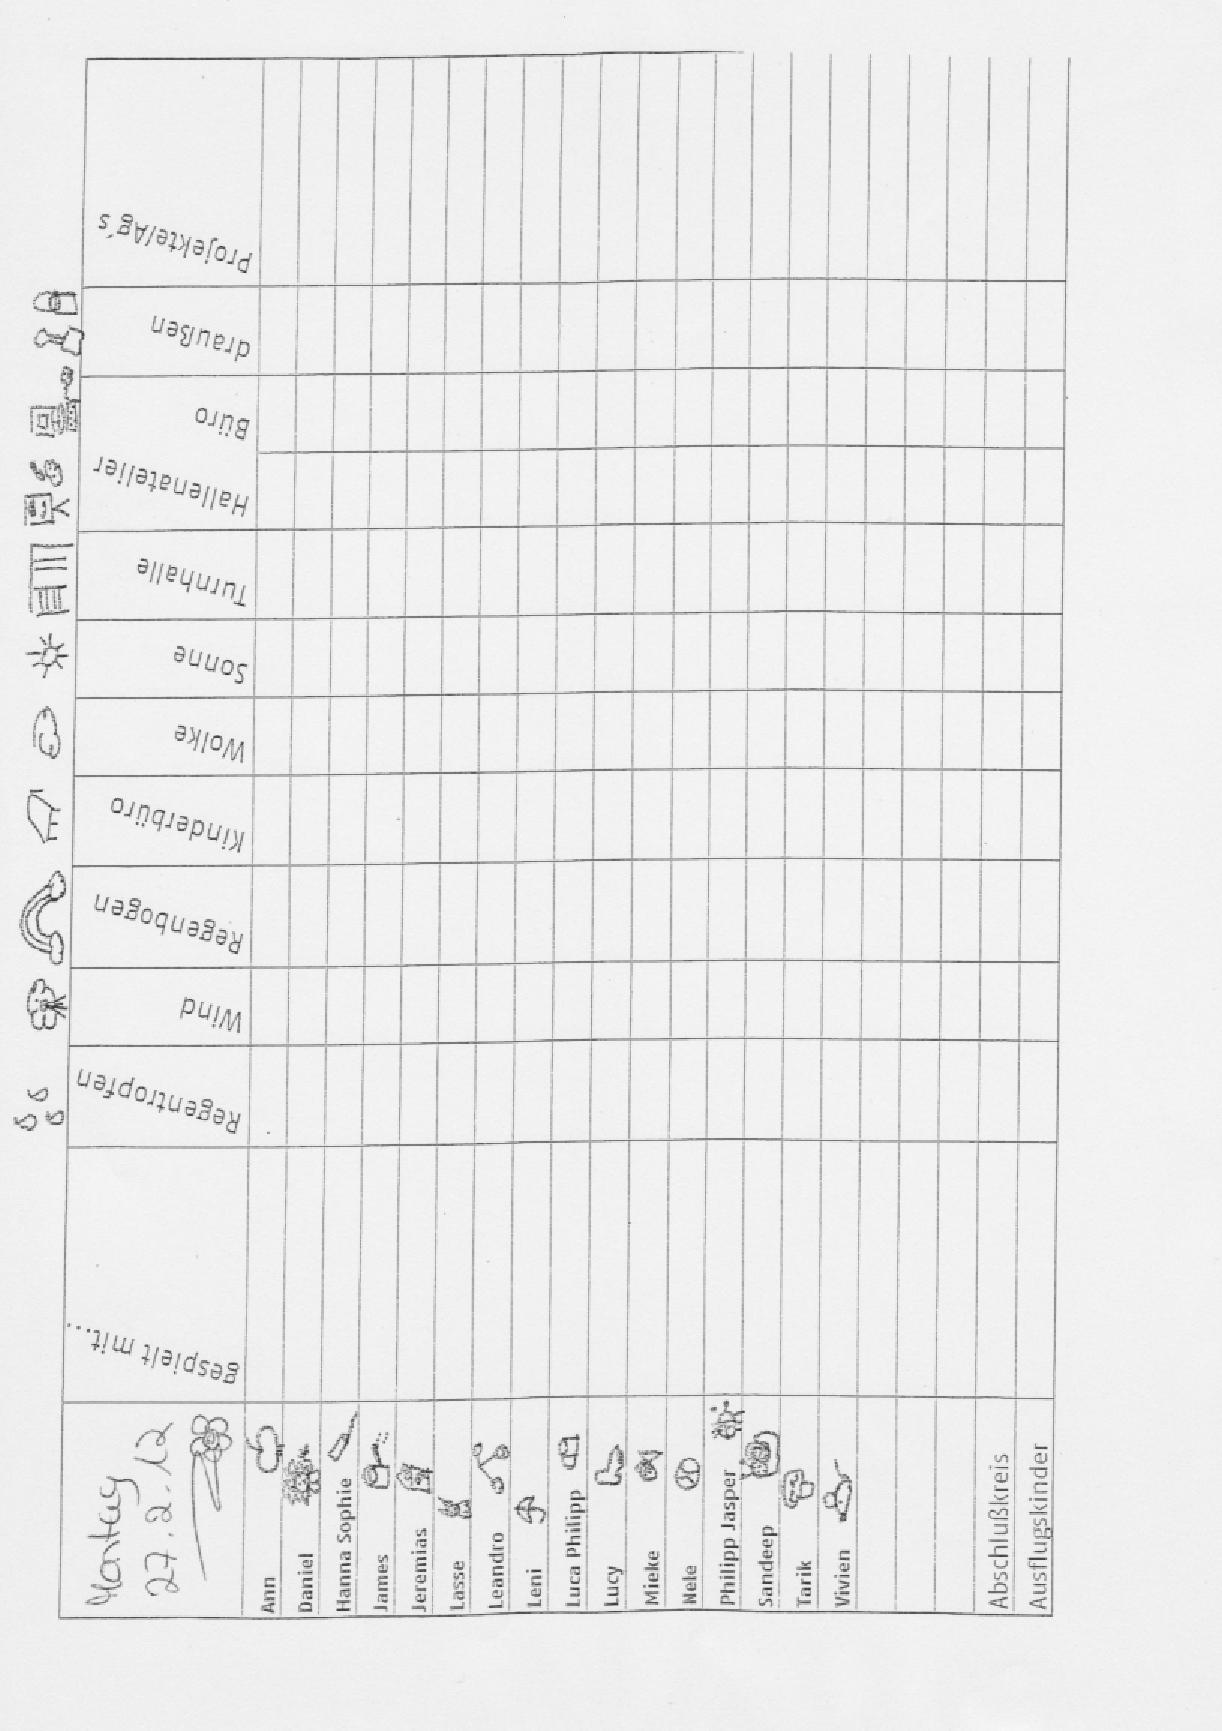
\includepdf[pages=-, addtotoc={1,chapter,0,Kinderankreuzliste,chap:anhang_1}, scale=0.80, offset=6mm -5mm]{anhang_1.pdf}
% 
% \includepdfset{pagecommand={\pagestyle{scrheadings}}}
% 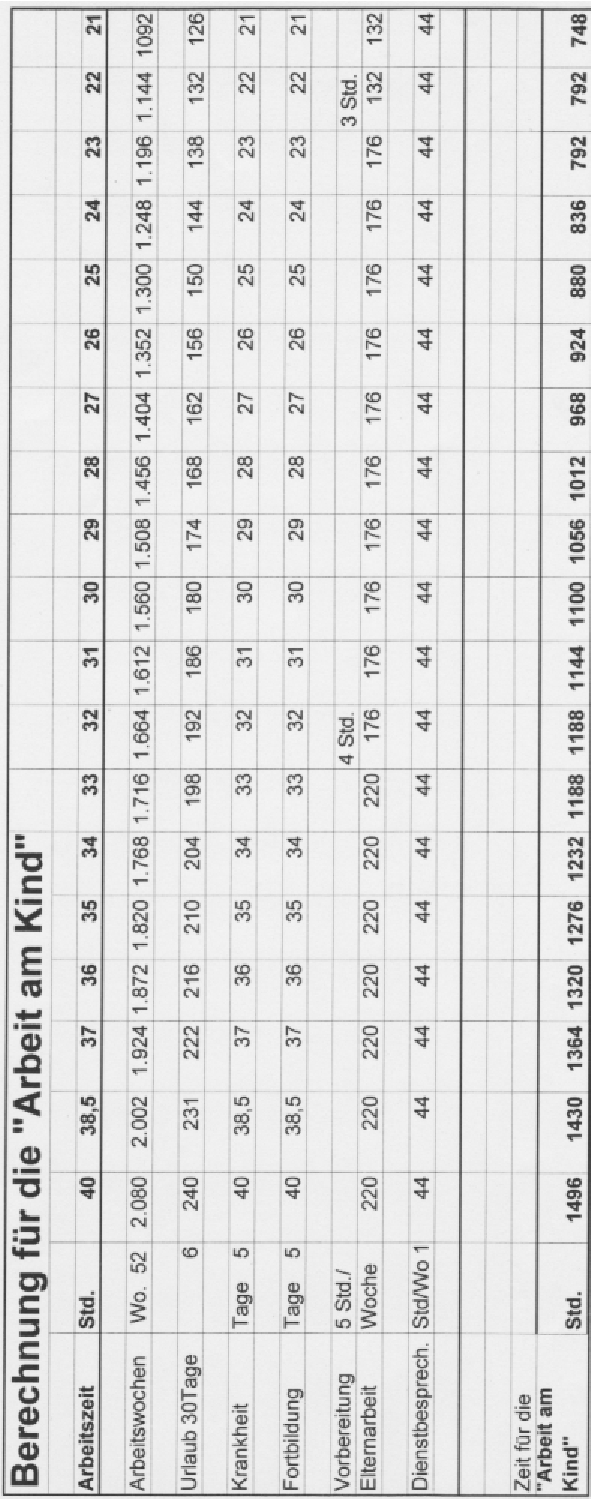
\includepdf[pages=-, addtotoc={1,chapter,0,Berechnung f�r die Arbeit am Kind,chap:anhang_2}, scale=0.80, offset=6mm -5mm]{anhang_2.pdf} 
% 
% \includepdfset{pagecommand={\pagestyle{scrheadings}}}
% 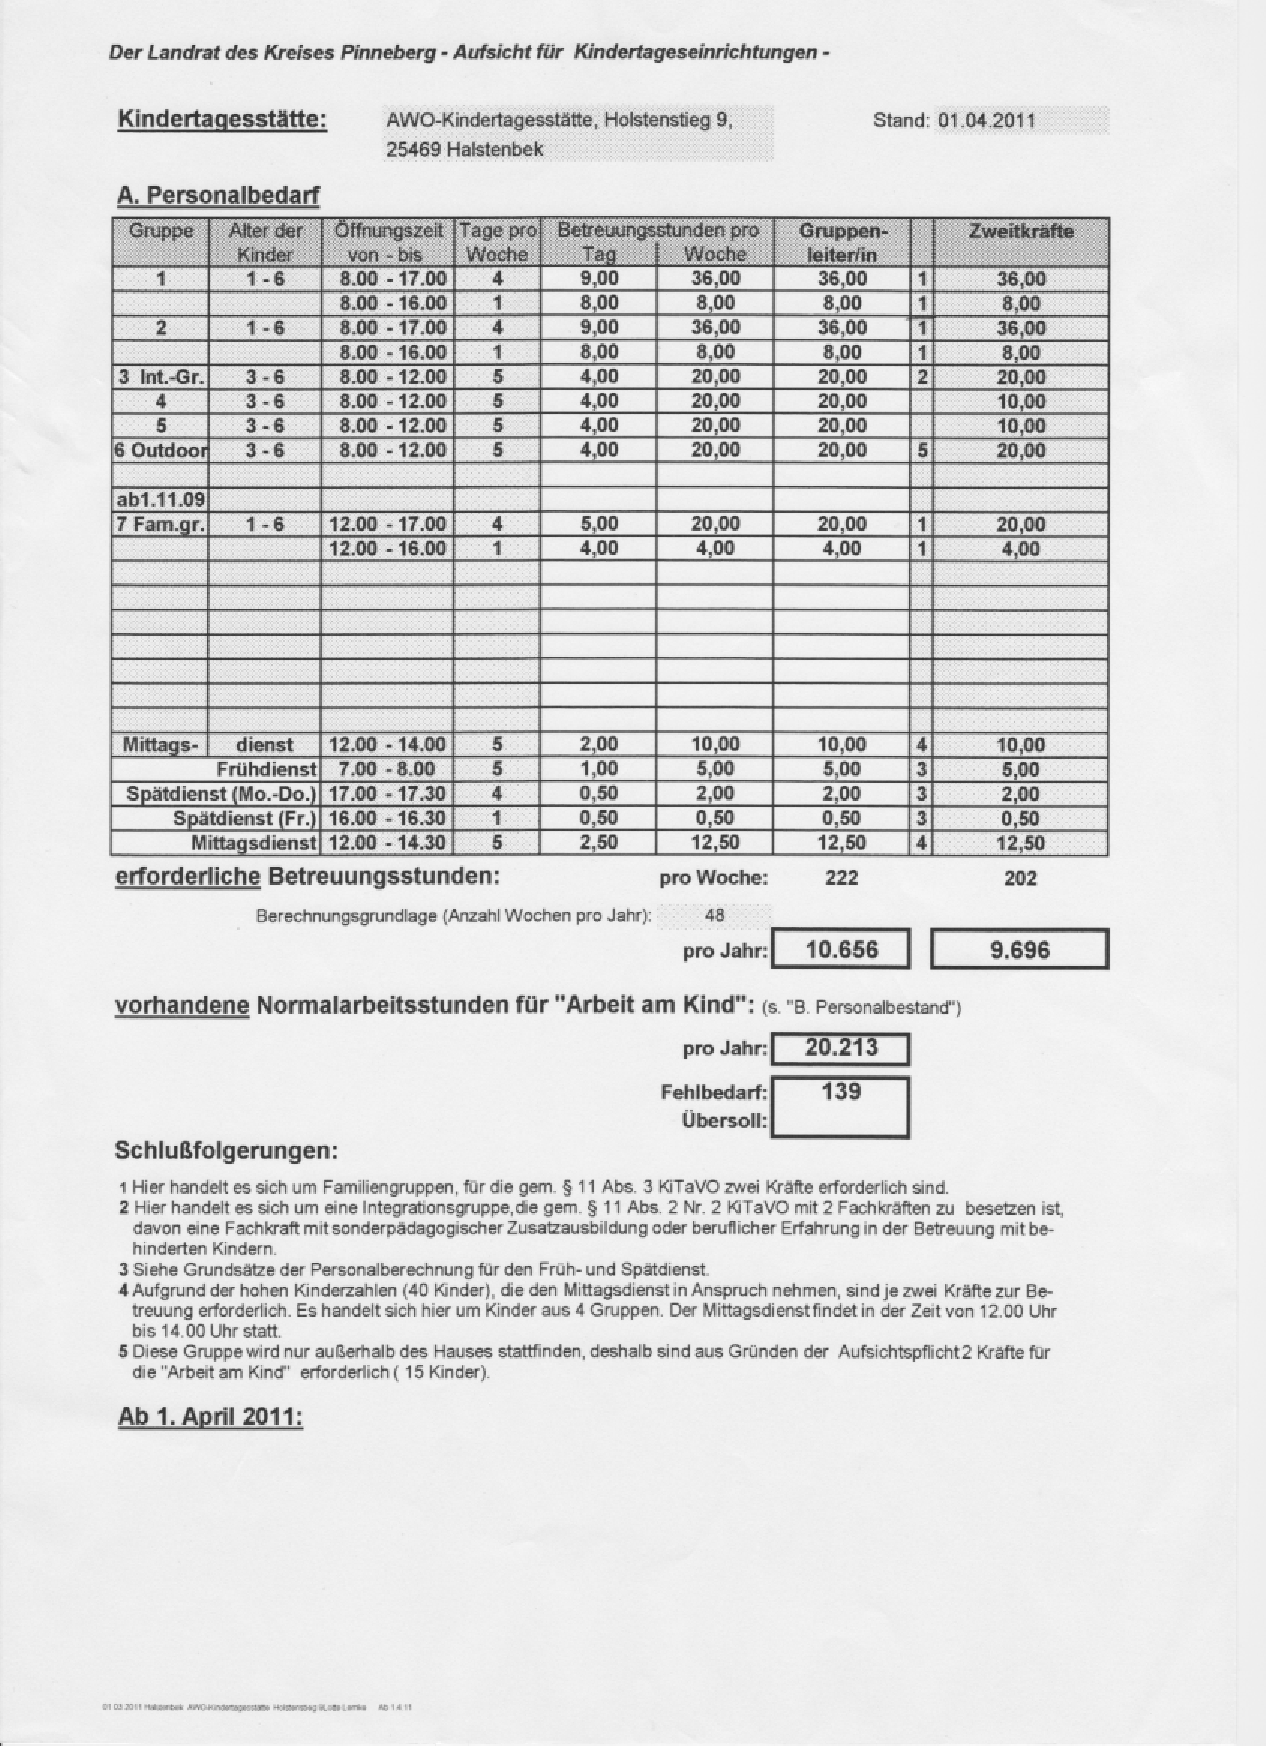
\includepdf[pages=-, addtotoc={1,chapter,0,Personalbedarf,chap:anhang_3}, scale=0.80, offset=6mm -5mm]{anhang_3.pdf}
% 
% \includepdfset{pagecommand={\pagestyle{scrheadings}}}
% 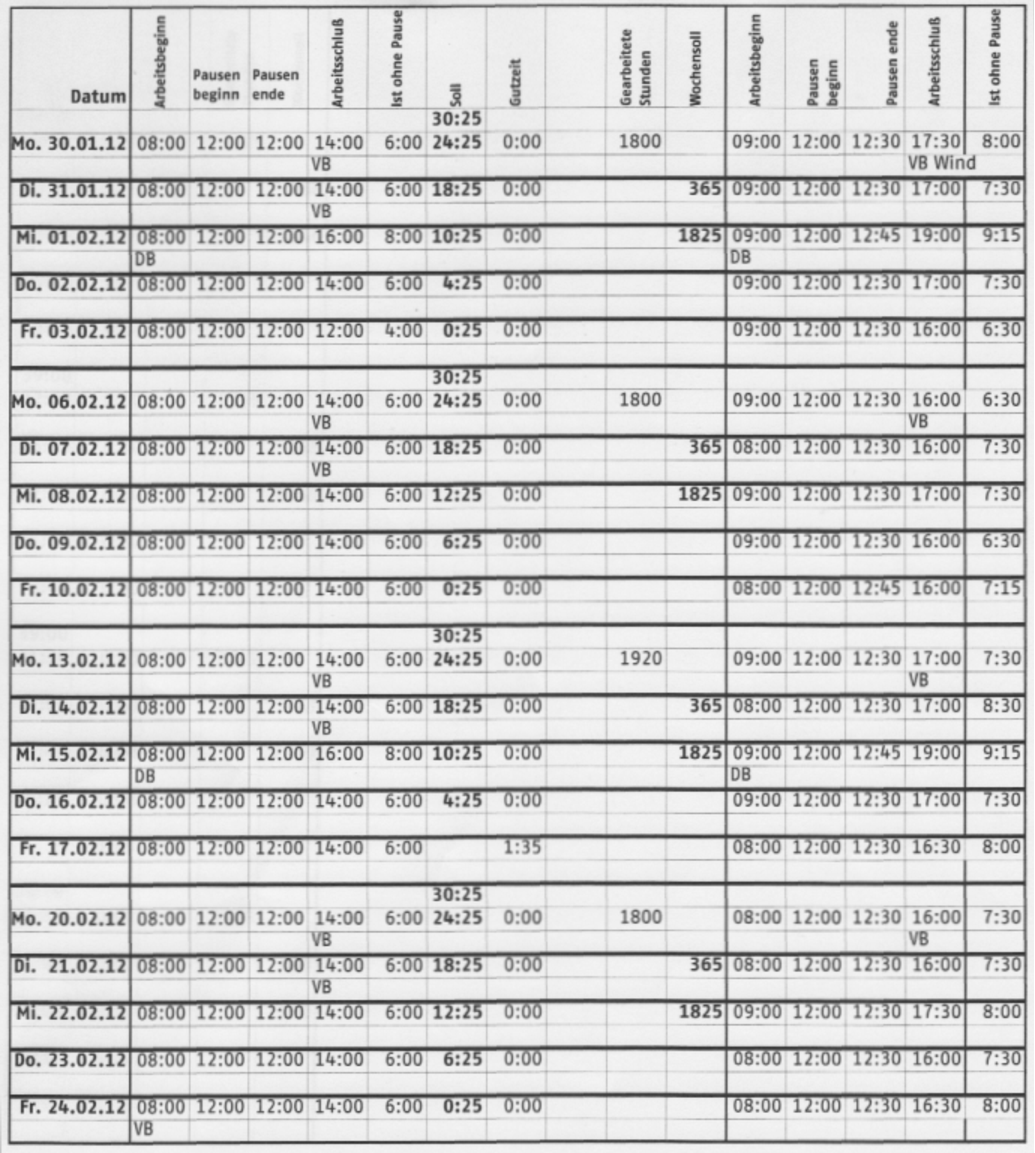
\includepdf[pages=-, addtotoc={1,chapter,0,Dienstplanberechnung,chap:anhang_4}, scale=0.80, offset=6mm -5mm]{anhang_4.pdf}
% 
% \includepdfset{pagecommand={\pagestyle{scrheadings}}}
% 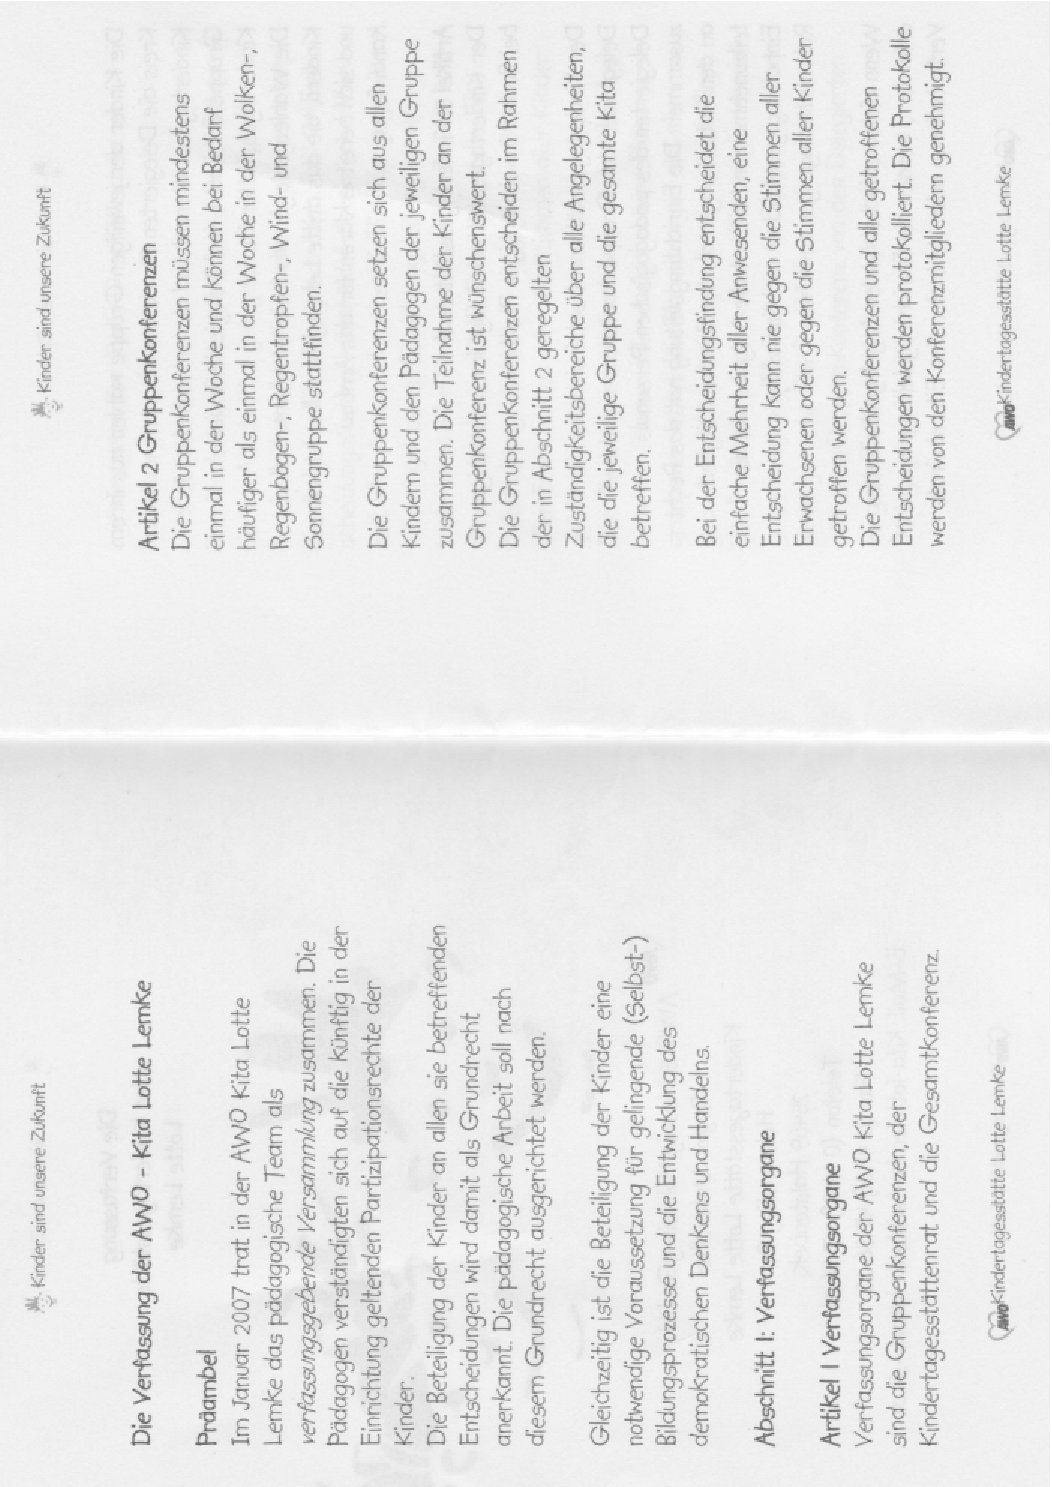
\includepdf[pages=-, addtotoc={1,chapter,0,Verfassung der KiTa,chap:anhang_5}, scale=0.80, offset=6mm -5mm]{anhang_5.pdf}
% 
% \includepdfset{pagecommand={\pagestyle{scrheadings}}}
% 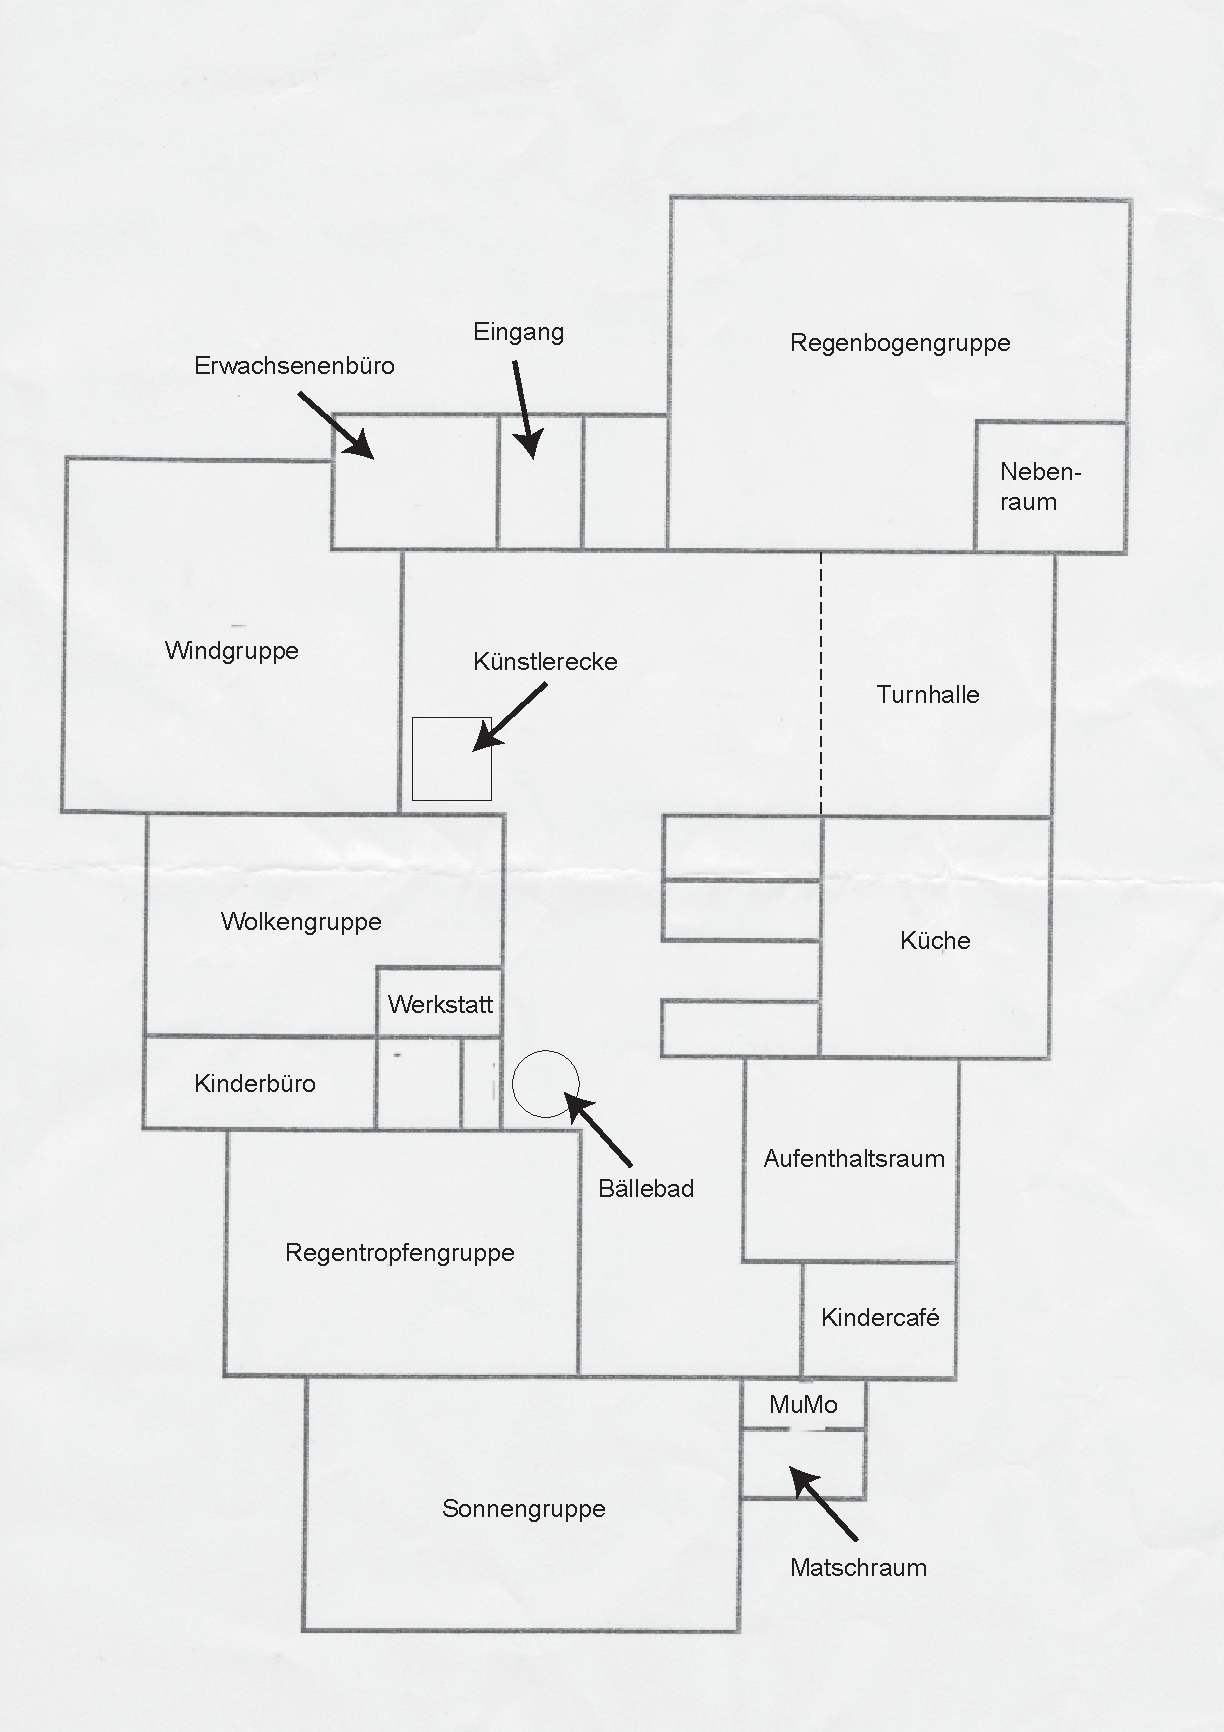
\includepdf[pages=-, addtotoc={1,chapter,0,Grundriss der KiTa,chap:anhang_6}, scale=0.80, offset=6mm -5mm]{anhang_6.pdf}
% 
% \includepdfset{pagecommand={\pagestyle{scrheadings}}}
% 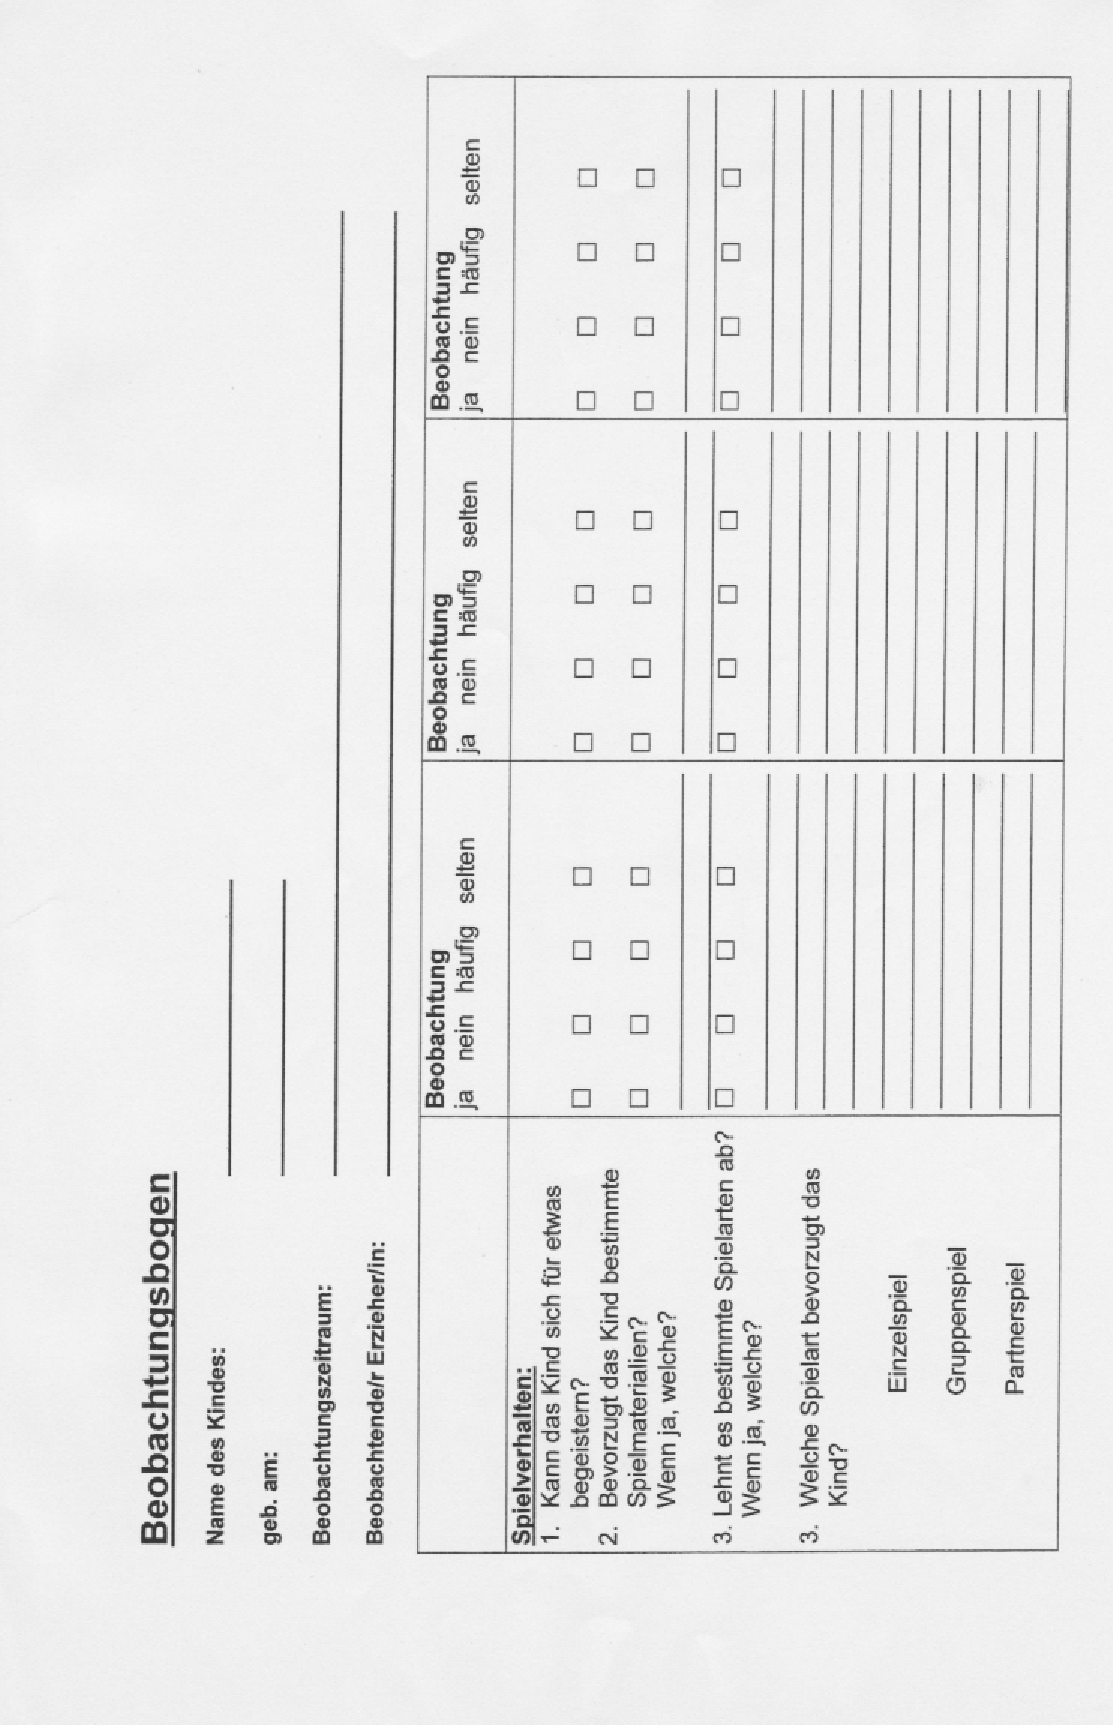
\includepdf[pages=-, addtotoc={1,chapter,0,Beobachtungsbogen,chap:anhang_7}, scale=0.80, offset=6mm -5mm]{anhang_7.pdf}
% 
% \includepdfset{pagecommand={\pagestyle{scrheadings}}}
% 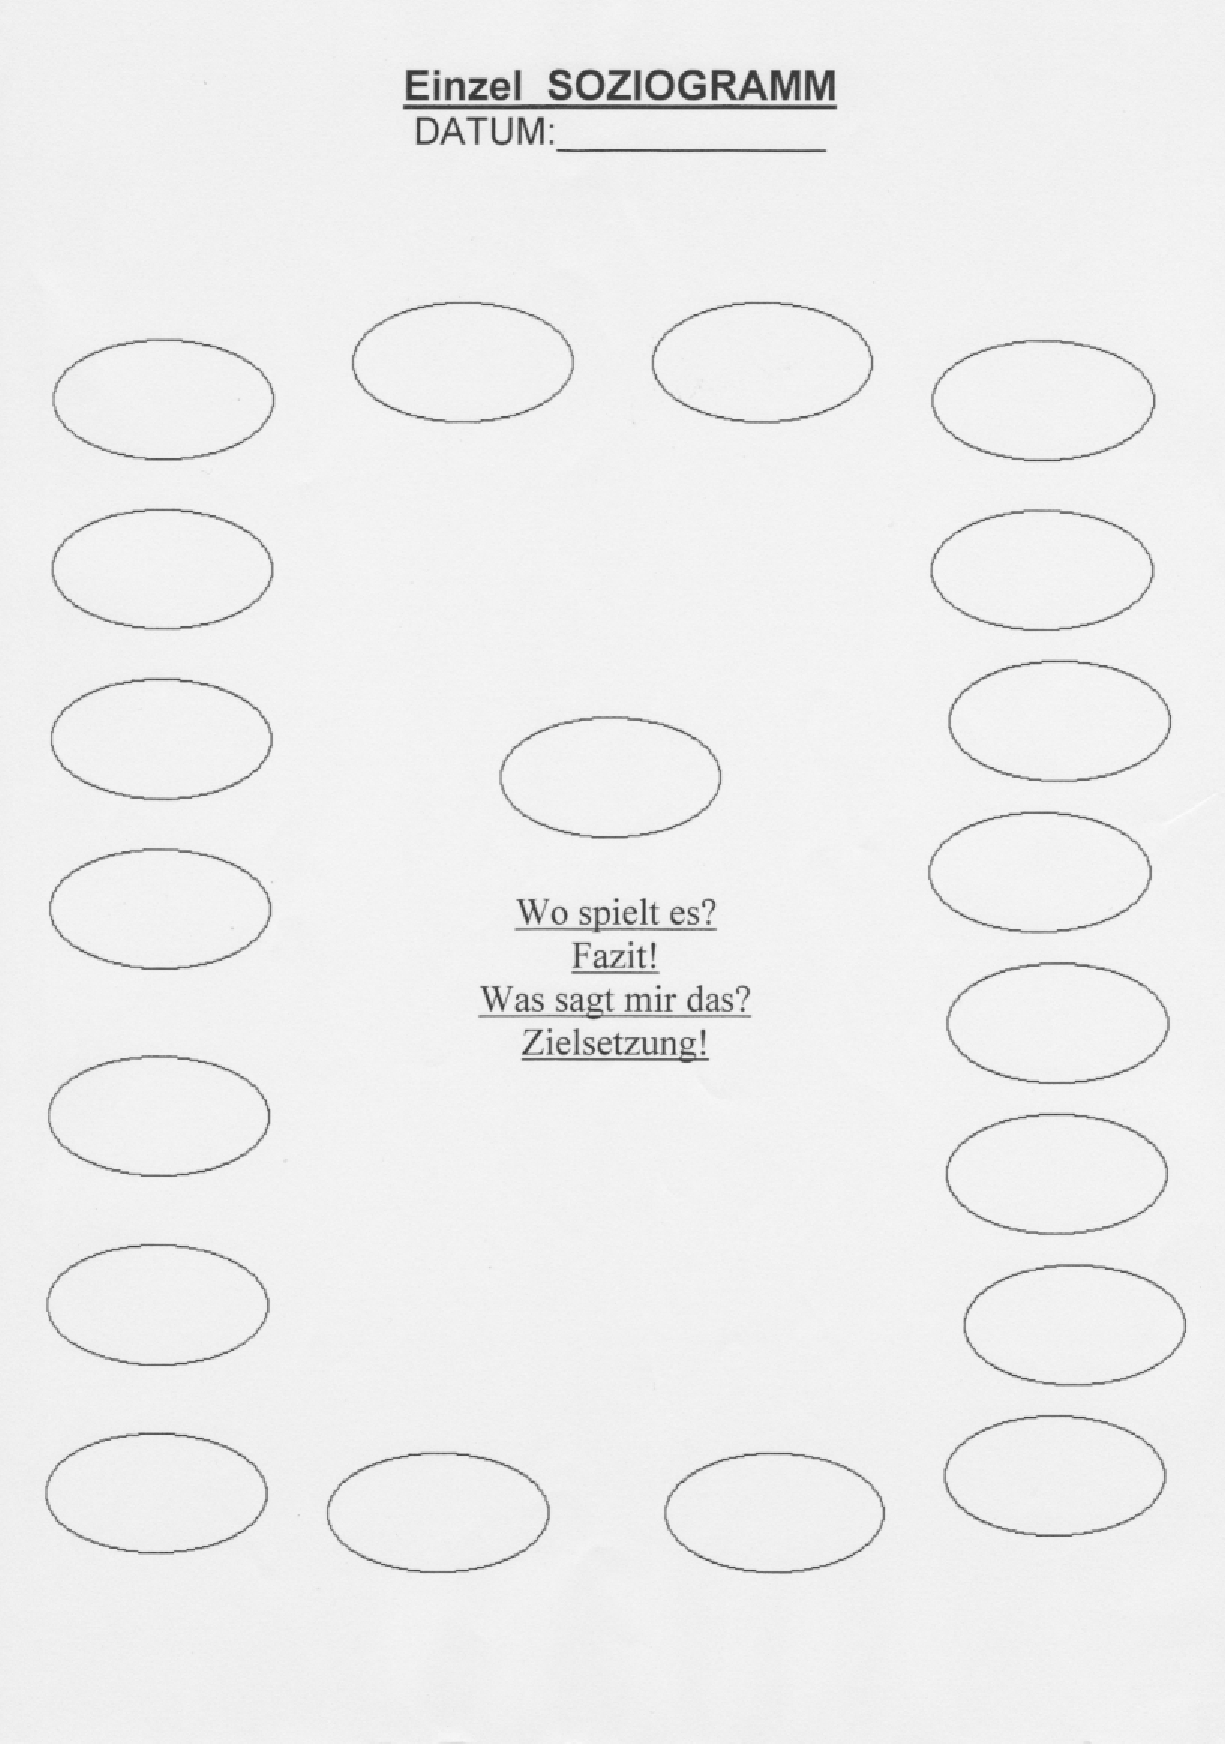
\includepdf[pages=-, addtotoc={1,chapter,0,Einzel Soziogramm,chap:anhang_8}, scale=0.80, offset=6mm -5mm]{anhang_8.pdf}
% 
% \includepdfset{pagecommand={\pagestyle{scrheadings}}}
% 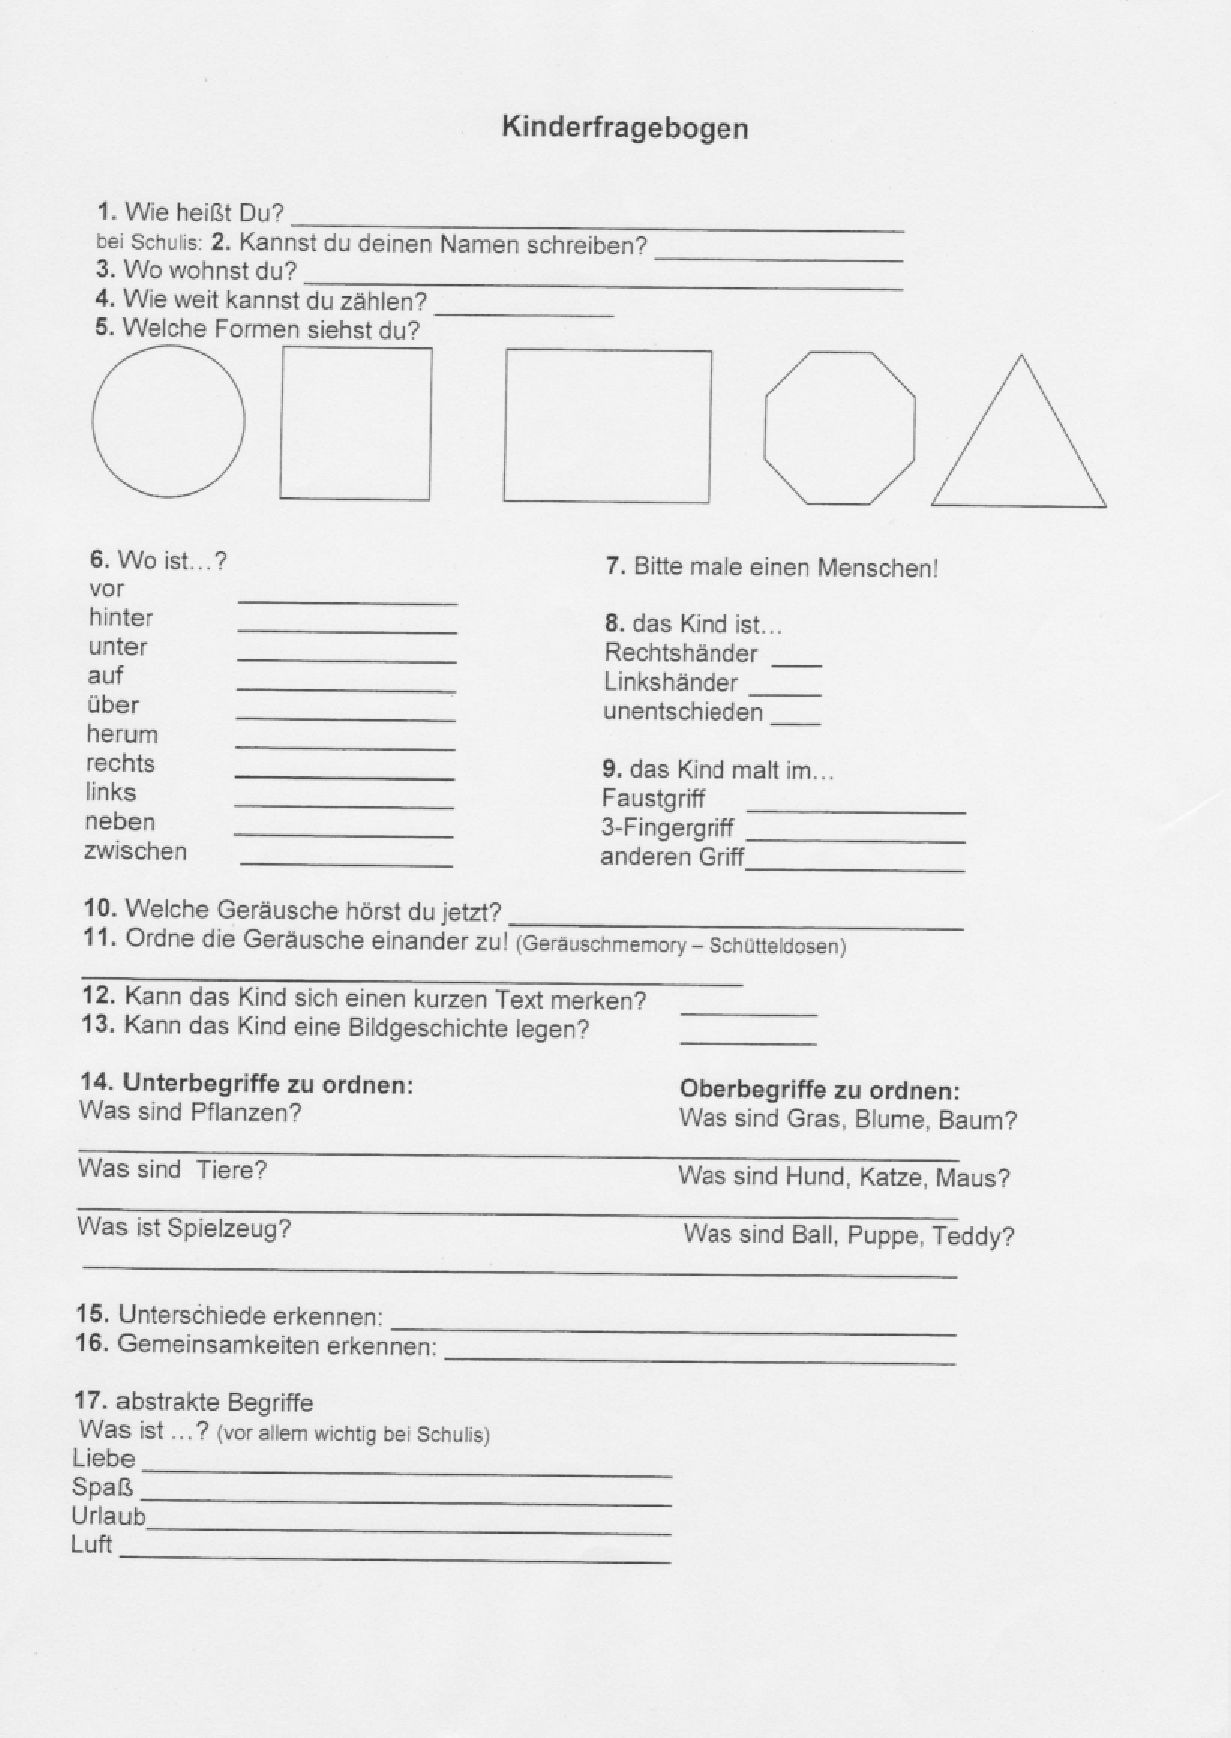
\includepdf[pages=-, addtotoc={1,chapter,0,Kinderfragebogen,chap:anhang_9}, scale=0.80, offset=6mm -5mm]{anhang_9.pdf}
% 
% \includepdfset{pagecommand={\pagestyle{scrheadings}}}
% 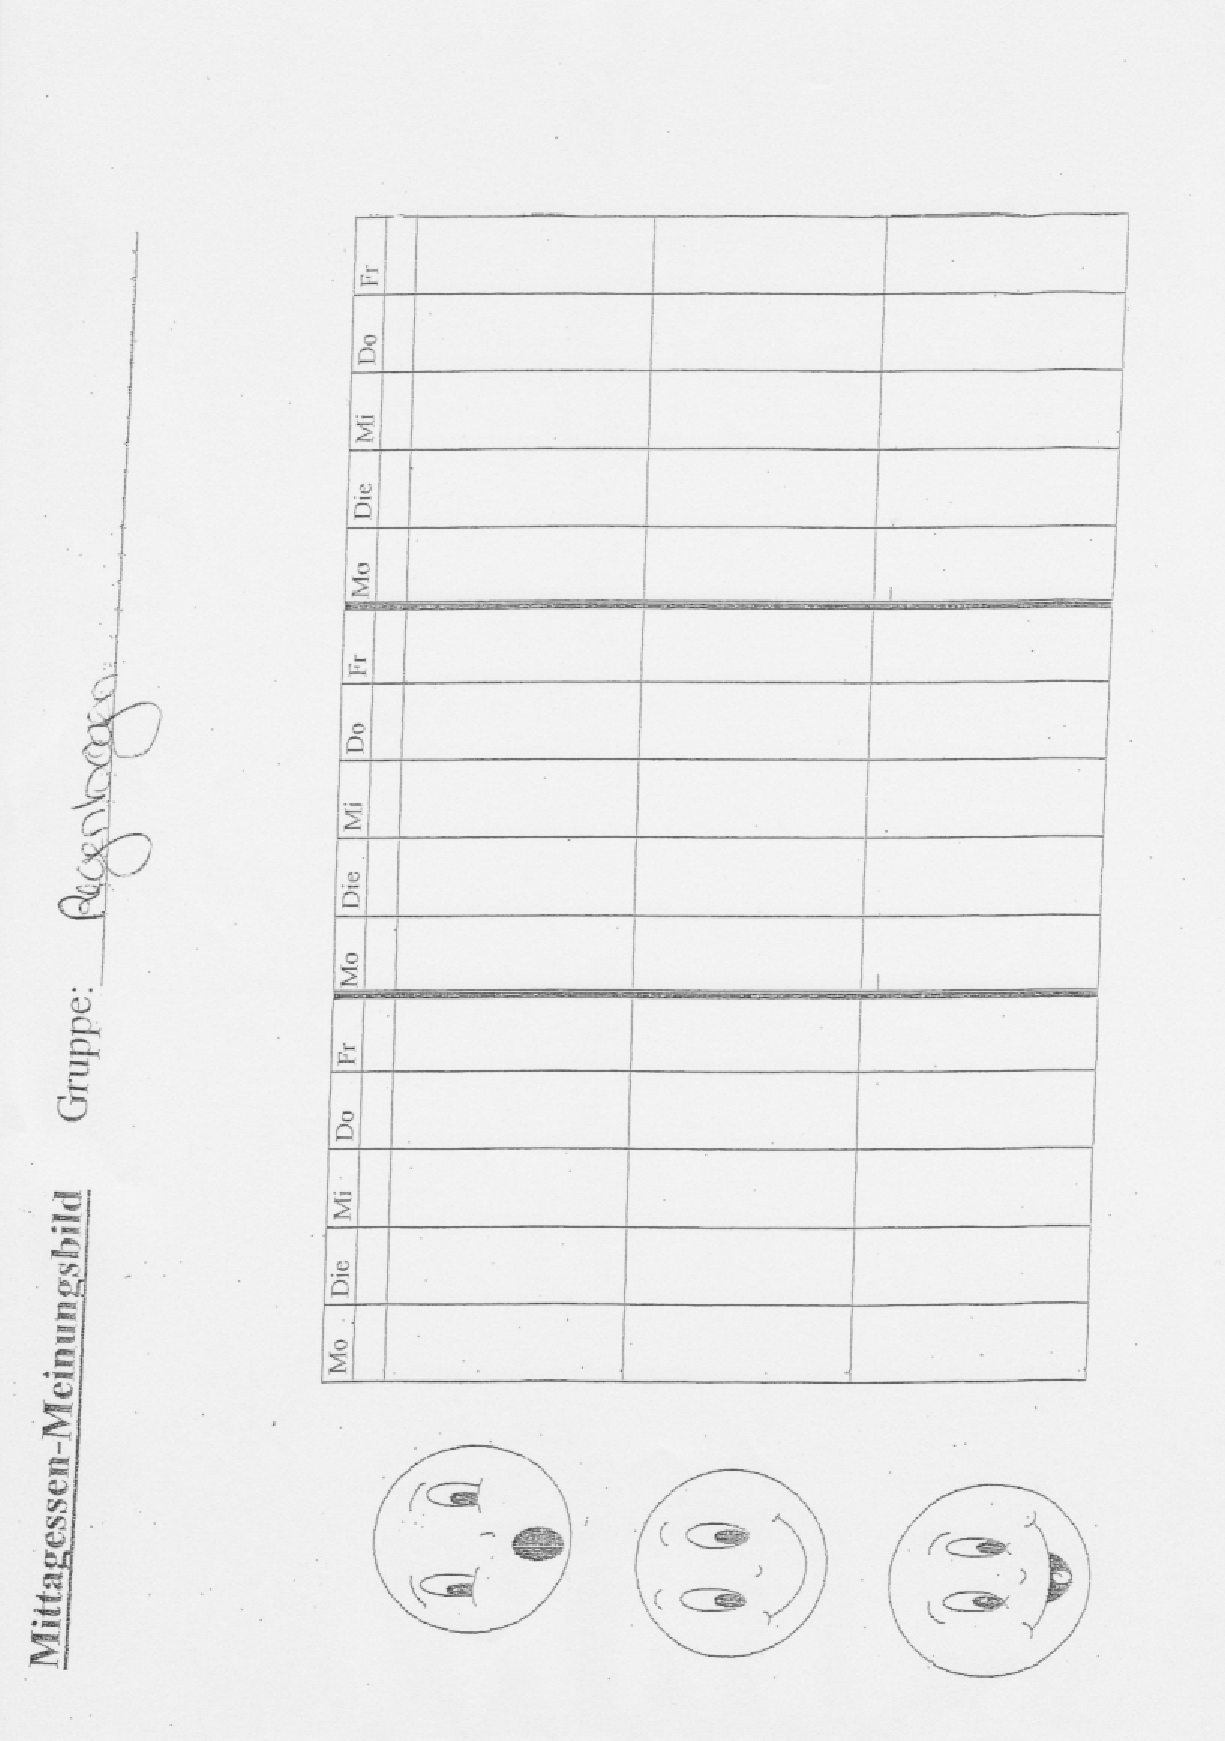
\includepdf[pages=-, addtotoc={1,chapter,0,Meinungsbild Mittagessen,chap:anhang_10}, scale=0.80, offset=6mm -5mm]{anhang_10.pdf}

% bibliography and other stuff
\backmatter
% \pagenumbering{arabic}
\typeout{===== Section: Literaturverzeichnis}
\cleardoublepage  
\phantomsection
\addcontentsline{toc}{chapter}{Literaturverzeichnis}
\bibliographystyle{natdin}
\bibliography{literatur}

% \typeout{===== Section: Glossar}
% \renewcommand{\glossaryname}{Glossar}
% \cleardoublepage  
% \phantomsection
% \addcontentsline{toc}{chapter}{Glossar}
% \clearpage
% \printglossaries

%% index
% \typeout{===== Section: Index}
\cleardoublepage  
% \phantomsection
% \addcontentsline{toc}{chapter}{Index}
% \printindex






% \HAWasurency

\end{document}
